\documentclass[11pt, oneside]{article} 
\usepackage{amsmath, amsthm, amssymb, calrsfs, wasysym, verbatim, bbm, color, graphics, graphicx, geometry}
\usepackage[most]{tcolorbox}
\usepackage{xcolor}
\usepackage{framed}
\colorlet{shadecolor}{blue!15}
\graphicspath{ {./figs} }

\geometry{tmargin=.75in, bmargin=.75in, lmargin=.75in, rmargin = .75in}  

\newcommand{\R}{\mathbb{R}}
\newcommand{\C}{\mathbb{C}}
\newcommand{\Z}{\mathbb{Z}}
\newcommand{\N}{\mathbb{N}}
\newcommand{\Q}{\mathbb{Q}}
\newcommand{\Cdot}{\boldsymbol{\cdot}}

\newtheorem{thm}{Theorem}
\newtheorem{defn}{Definition}
\newtheorem{conv}{Convention}
\newtheorem{rem}{Remark}
\newtheorem{lem}{Lemma}
\newtheorem{cor}{Corollary}
\newtheorem{exa}{Example}


\title{Hidr\'aulica B\'asica [2015961] \\ \textbf{Tema \# 1: Flujo real y disipaci\'on de energ\'ia}}
\author{\textbf{Luis Alejandro Morales (Ph.D)}\\ \vspace{0.4cm} Profesor Asistente \\ Universidad Nacional de Colombia-Bogot\'a\\Facultad de Ingenier\'ia \\ Departamento de Ingenieria Civil y Agr\'icola}
%\date{Periodo 2022-II}
\date{}

\begin{document}

\maketitle
\tableofcontents

%\vspace{.25in}

%%%%%%%%
\section{Fluido ideal y fluido real} % From Street
\subsection{Flujo ideal}
Un \textbf{fluido ideal} es un fluido hipot\'etico en donde  se asume que el fluido no tiene viscosidad por lo tanto la \emph{ley de viscosidad de newton} 

\begin{equation}
\tau = \mu \frac{du}{dy}
\label{vis}
\end{equation}

en donde $\tau$ es el esfuerzo de corte, $\mu$ es la viscosidad din\'amica y $u=f(y)$ es la velocidad del flujo, no es aplicable. Esto quiere decir que la fricci\'on en el flujo es despreciable por lo tanto  no existen esfuerzos de corte entre capas ni con los contornos, lo que implica que no hay disipaci\'on de energ\'ia debido a la fricci\'on ni formaci\'on de remolinos. En un fluido ideal las part\'iculas se mueven unas sobre otras sin ning\'un tipo resistencia, sometidas a fuerzas hidroest\'aticas aplicadas sobre su superficie. El movimiento y la aceleraci\'on de dichas part\'iculas se presenta gracias al desbalance de fuerzas actuantes de acuerdo con la \emph{segunda ley de Newton}. La suposisi\'on de fluido ideal es de gran ayuda para el an\'alisis de problemas pr\'acticos en ingenier\'ia en donde las fuerzas viscosas son despreciables dando resultados precisos. Por ejemplo si se quiere determinar la fuerza de levantamiento del ala de un avi\'on es posible asumir un fluido ideal, sin embargo, dicha suposisi\'on no ser\'ia correcta si se quisiera determinar la fuerza de arrastre sobre el ala de un avi\'on. Asumiendo el flujo de part\'iculas de fluido ideal e \emph{incompresible} (en donde la densidad no cambia) y de acuerdo con la \emph{segunda ley de Newton}, se deduce la \emph{ecuaci\'on de Bernoulli}:

\begin{equation}
\frac{p}{\gamma} + \frac{V^2}{2g}+z = H = Constante
\label{bernu}
\end{equation}

donde $p$ es la presi\'on (absoluta o manom\'etrica), $V$ es la velocidad media del flujo, $z$ es la altura del sistema con respecto a un nivel de referencia y $H$ es la cabeza de energ\'ia total en una secci\'on del flujo la cual es constante ($H_1 = H_2 $) y equivale a la suma de la \emph{cabeza de energ\'ia de presi\'on} ($p/\gamma$), \emph{cabeza de energ\'ia cin\'etica} ($V^2 /2g$) y \emph{cabeza de energ\'ia potencial} ($z$). Note que al termino $\frac{p}{\gamma} + \frac{V^2}{2g}$ se le conoce como \emph{cabeza de presi\'on din\'amica} la cual se puede medir usando un \emph{tubo Pitot}. La ecuaci\'on de Bernoulli, puede ser expresada gr\'aficamente a trav\'es de la \emph{l\'inea de energ\'ia} (LE=$H$) y \emph{l\'inea de gradiente hidr\'aulico} (LGH = $p/\gamma + z$).

La inclusi\'on (a trav\'ez de una \emph{bomba}) o la extracci\'on (a trav\'es de una \emph{turbina}) de energ\'ia a un flujo de un fluido ideal da lugar a una forma mas completa de la ecuaci\'on de Bernoulli conocida tambi\'en como la \emph{ecuaci\'on de trabajo-energia}:

\begin{equation}
\frac{p_1}{\gamma} + \frac{V_1^2}{2g} + z_1 + h_B =\frac{p_2}{\gamma} + \frac{V_2^2}{2g} + z_2 + h_T
\end{equation}

donde $h_B$ es la energ\'ia suministrada por una bomba y $h_T$ es la eneg\'ia sustra\'ida por una turbina. La potencia hidr\'aulica ($P_H$) suministrada (bomba) al flujo o extra\'ida (turbina) del flujo, se calcula como:

\begin{equation}
P_H = \gamma h Q
\end{equation}
donde $h$ es la cabeza de energ\'ia mec\'anica ($h_B$ o $h_T$) y $Q$ es el caudal. La \emph{potencia nominal (o mec\'anica)} ($P_n$) es:
\begin{equation}
P_n = \frac{P_H}{\eta}
\end{equation}
donde $\eta$ es la eficiencia de la bomba.

 
\subsection{Flujo real}
En un \textbf{flujo real} su movimiento es controlado por las \emph{fuerzas de fricci\'on} y las \emph{fuerzas turbulentas}. Esto quiere decir que para mover un flujo real, es necesario realizar trabajo sobre el flujo para vencer estos esfuerzos y dicha energ\'ia se convierte en calor. Es por esto que en un \emph{flujo laminar} las capas de fluido adyancentes se mueven a velocidades diferentes en funci\'on de la transmisi\'on de esfuerzos de corte en la interface. Lo mismo ocurre en las fronteras solidas en donde la fricci\'on de las paredes son transmitidas a las capas de flujo haciendo que su velocidad aumente a medida que se alejan de las paredes. El grado de ''pegajosidad'' depende de la viscosidad del fluido. Los fluidos reales tambi\'en se conocen como \emph{flujos Newtonianos} por que siguen la ley de visosidad de Newton (ver Ecuaci\'on~\ref{vis}).

En el caso de \emph{flujos turbulentos}, flujos a velocidades altas generalmente, los esfuerzos viscosos generan vortices en el flujo. Si a las ecuaciones de \emph{Euler} se le adicionan los t\'erminos debido a los esfuerzos de corte, se obtienen las \emph{ecuaciones de Navier-Stokes} las cuales son un sistema de ecuaciones diferenciales parciales no lineales y de segundo grado que describen el movimiento de flujos reales, compresibles o incompresibles y permanentes o no permanentes. Las ecuaciones de Navier-Stokes para fluidos incompresibles son:

\begin{equation}
-\frac{1}{\rho}\frac{\partial}{\partial x}(p + \gamma h) + \nu \nabla^2 u = \frac{du}{dt}
\label{nast1}
\end{equation}

\begin{equation}
-\frac{1}{\rho}\frac{\partial}{\partial y}(p + \gamma h) + \nu \nabla^2 v = \frac{dv}{dt}
\label{nast2}
\end{equation}

\begin{equation}
-\frac{1}{\rho}\frac{\partial}{\partial z}(p + \gamma h) + \nu \nabla^2 w = \frac{dw}{dt}
\label{nast3}
\end{equation}

donde $\nu$ es la viscosidad cinem\'atica (constante para este caso), $\frac{d}{dt}=u\frac{\partial}{\partial x}+v\frac{\partial}{\partial y}+w\frac{\partial}{\partial z}+\frac{\partial}{\partial t}$ es la derivada total y $\nabla^2 = \frac{\partial^2}{\partial x^2} + \frac{\partial^2}{\partial y^2} + \frac{\partial^2}{\partial z^2}$ (laplaciano). Para un fluido no viscoso, las ecuaciones de Navier-Stokes se convierten en las \emph{ecuaciones de Euler}.


Los efectos de los esfuerzos viscosos, son mas notorios en cercan\'ias a las fronteras solidas (e.g fondo del canal o paredes de una tuber\'ia); dicha regi\'on es conocidad como \emph{capa l\'imite}. 


%%%%%%%%
\section{Capa limite en flujo a presi\'on} % From Street
En un flujo real  la \textbf{capa l\'imite} es una porci\'on de la secci\'on de flujo en donde los esfuerzos debido a la fricci\'on (viscosos) est\'an confinados o cobran gran importancia y en donde el flujo es \emph{rotacional} $\vec{\nabla} \times  \vec{U} \neq 0$. Esto quiere decir por fuera de la capa l\'imite la viscosidad del fluido es inoperativa y el flujo es \emph{irrotacional}  $\vec{\nabla} \times  \vec{U} = 0$.

Un \emph{flujo a presi\'on} o flujo interno es aquel que viaja por un conducto y ocupa toda su secci\'on transversal (ver figura~\ref{ttub}). El movimiento del flujo en el conducto se da por el gradiente de presi\'on entre dos puntos en el conducto separadas una distancia $L$. Dicho gradiente se presenta gracias a la perdida de energ\'ia a lo largo de $L$ debido a los esfuerzos de fricci\'on y a la separaci\'on del flujo.  

\begin{figure}[h]
\centering
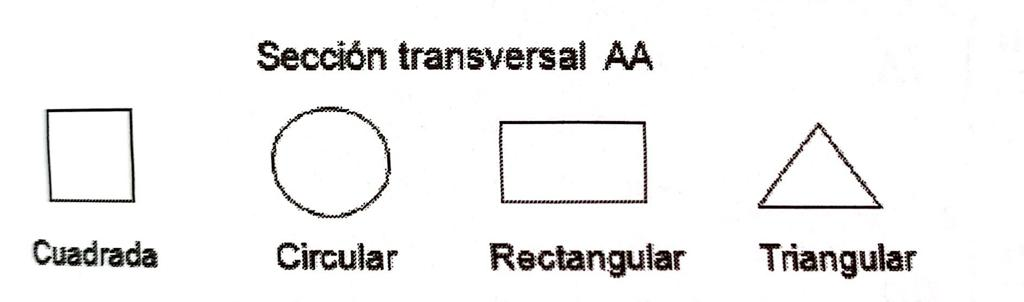
\includegraphics[width=8cm]{ttub.jpeg}
\caption{Tipos comunes de secciones transversales de tuber\'ias (tomado de \cite{agudelo2011mecanica}).}
\label{ttub}
\end{figure}

Si se tiene un tanque grande del cual se conecta en la parte baja una tuber\'ia (ver figura~\ref{cali}), los esfuerzos viscosos empiezan a crecer una vez el fluido ingresa a la tuber\'ia y por tanto la capa l\'imite ($\delta$) tambi\'en empieza a crecer a lo largo de la tuber\'ia. La zona inicial es una zona de flujo ideal en donde los esfuerzos viscosos son despreciales y por lo tanto la velocidades son uniformes. Una vez, el flujo sale de zona inicial, la capa l\'imite crece en una zona de \emph{flujo no establecido} en donde se desarrollan los esfuerzos de corte. Es posible que cuando la entrada a la tuber\'ia no se hace a trav\'es de una transici\'on suave, se presente separaci\'on del flujo de las paredes de la tuber\'ia generandose remolinos que viajan y desaparecen a lo largo de la zona de flujo no establecido y \emph{presiones negativas} a velocidades muy altas. Una vez las capas l\'imites alrededor y crecientes en direcci\'on del flujo se encuentran es cuando se tiene un \emph{flujo establecido} o flujo real gobernado por los esfuerzos de corte con una distribuci\'on no uniforme de velocidades.
  
\begin{figure}[h]
\centering
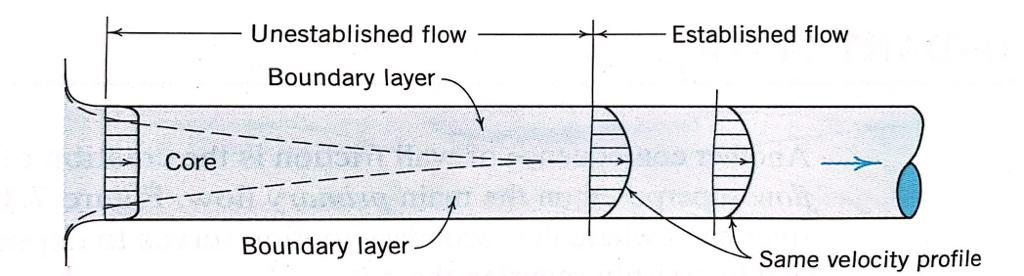
\includegraphics[width=8cm]{cali.jpeg}
\caption{Desarrollo de la capa l\'imite a lo largo de una tuber\'ia (tomado de \cite{street471elementary}).}
\label{cali}
\end{figure}

El mecanismo de crecimiento de la capa l\'imite se puede describir como sigue. Cuando el fluido entra a la tuber\'ia se desarrollan altos valores de $dv/dy$, donde $y$ es el eje vertical. Estos altos gradientes ocurren dentro de la capa l\'imite y son debido a los esfuerzos debido a la fricci\'on los cuales tratan de frenar el flujo. Dicha capa crece en la direcci\'on del flujo hasta el punto en el que se encuentran. A partir de este punto de encuentro la acci\'on de las fuerzas de friccion influencian el flujo y toda la secci\'on es rotacional.

El flujo dentro de la capa l\'imite puede ser laminar o turbulento. Si el numero de Reynolds $Re = \frac{Vd}{\nu}$, donde $V$ es la velocidad media del flujo, $d$ es el di\'ametro de la tuber\'ia y $\nu$ es la viscosidad cinem\'atica, es $Re < 2100$, se puede inferir que el \emph{flujo laminar establecido} resulta del crecimiento de la capa l\'imite laminar. En este caso la longitud que toma el establecimiento de este flujo es $\frac{x}{d} \approx \frac{Re}{20}$. Si el $Re$ aumenta levemente el flujo ser\'a laminar a lo largo de $\frac{x}{d} \approx \frac{Re}{20}$ y luego sera transisional antes de que el flujo este establecido. Si $Re >> 2100$ la capa l\'imite ser\'a turbulenta. Para $Re$ altos, en casos pr\'acticos se puede decir que la longitud $x$ de la zona de flujo puede ser hasta $x \approx 100 d$. Sin embargo, el flujo es establecido para valores mayores a $\frac{x}{d} \approx 20$. De acuerdo con esto, es posible notar que la energ\'ia en un flujo establecido disminuye a lo largo de la tuber\'ia. Note que la energ\'ia debido a la cabeza de presi\'on disminuye a lo largo de la tuber\'ia debido a los esfuerzos de corte generados por la fricci\'on dentro del flujo establecido (ver figura~\ref{fifr}). 
  
\begin{figure}[h]
\centering
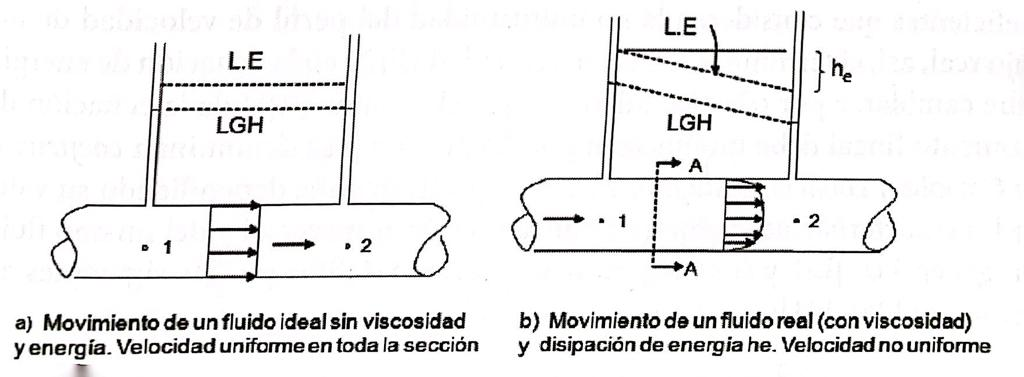
\includegraphics[width=8cm]{fifr.jpeg}
\caption{L\'inea de gradiente hidra\'aulico (LGH) y de energ\'ia (LE) en un a) fluido ideal y en un b) fluido real (tomado de \cite{agudelo2011mecanica}).}
\label{fifr}
\end{figure}

%%%%%%%%
\section{Esfuerzo de corte y perdidas de cabeza de energ\'ia} % From Street
Los esfuerzos de corte son producidos debido a la turbulencia del flujo o la viscosidad del fluido lo que con lleva a una resistencia al flujo que se traduce en perdidas de energ\'ia. Una pregunta clave, que se derivar\'ia es ¿Cuales son los efectos de las fuerzas de fricci\'on sobre la superficie de un volumen de control, por ejemplo,  en una tuber\'ia?. Para esto, analizaremos los esfuerzos de corte ($\tau$) en un  flujo 1D compresible y permanente a trav\'es de la tuber\'ia inclinada de la figura~\ref{tau}.
   
\begin{figure}[h]
\centering
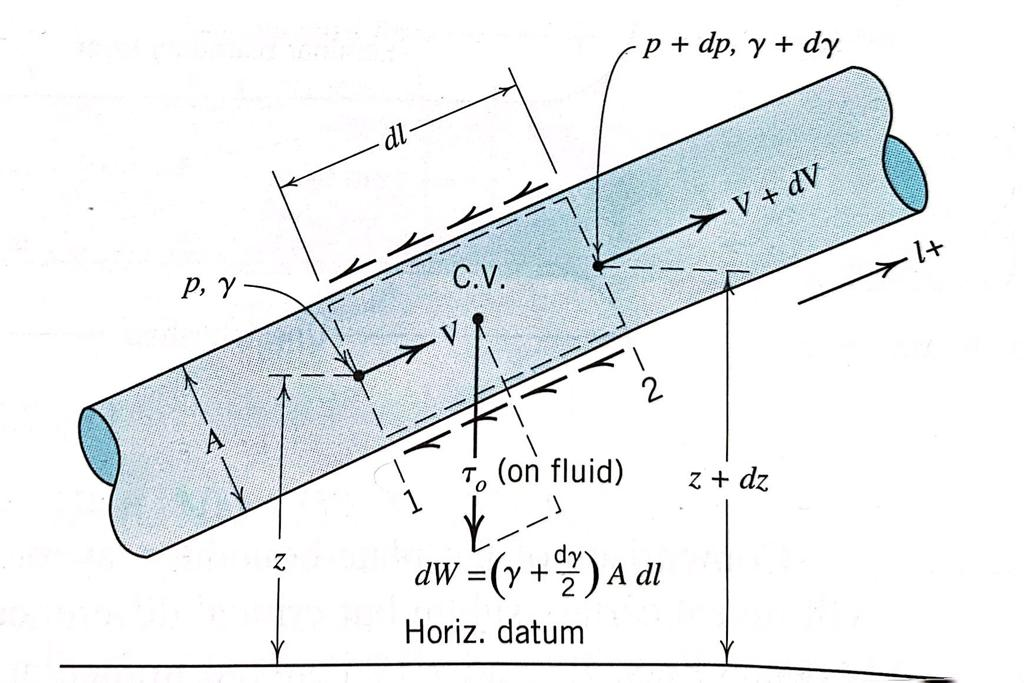
\includegraphics[width=8cm]{tau.jpeg}
\caption{Fuerzas actuantes sobre el volumen de control en la tuber\'ia inclinada (tomado de \cite{street471elementary}).}
\label{tau}
\end{figure}

Aplicando la \emph{ecuaci\'on de conservaci\'on de candidad de movimiento lineal} para las fuerzas actuantes en la direcci\'on del flujo sobre el volumen de control entre las secciones 1 y 2 en la  figura~\ref{tau}, tenemos que las fuerzas fundamentales que act\'uan son las \emph{fuerzas de presi\'on}, las \emph{fuerzas gravitacionales} y las \emph{fuerzas viscosas}. Por esto se tiene:

\begin{equation}
pA - (p+dp)A - \tau_{o} P dl - \left( \gamma + \frac{d \gamma}{2} \right)A dl \frac{dz}{dl} = (V+dV)^2 A (\rho +d \rho)- V^2 A \rho
\label{tau1}
\end{equation}

donde $V$ es la velocidad del flujo, $p$ es la presi\'on en la secci\'on, $P$ es el per\'imetro de la secci\'on, $A$ es el \'area de la secci\'on transversal, $\tau_{o}$ es el esfuerzo de corte en la superficie de control, $dl$ es la longitud del volumen de control, $dV$ es un cambio en la velocidad a trav\'es de $dl$, $dz$ es la diferencia de alturas entre las secciones 1 y 2, $\rho$ es la densidad del fluido, $\gamma$ es el peso espec\'ifico del fluido, $d \rho$ es un cambio de $\rho$ a trav\'es de $dl$ y $d \gamma$ es el cambio del peso espec\'ifico a lo largo de $dl$. Note que $\left( \gamma + \frac{d \gamma}{2} \right) A dl \frac{dz}{dl} = dW \frac{dz}{dl}$, donde $dW \frac{dz}{dl}$ es el peso del fluido en el volumen de control en la direcci\'on contraria del flujo, donde $\frac{dz}{dl}=\sin \theta$ y $\theta$ es el angulo de inclinaci\'on de la tuber\'ia. Teniendo en cuenta que entre 1 y 2 los efectos de turbinas y bombas son despreciables, dividiendo por $A\gamma$, donde $\gamma = \rho g$ y despreciando los terminos que contengan productos de diferenciales,  la ecuaci\'on~\ref{tau1} queda: 
 
\begin{equation}
\frac{dp}{\gamma} + d\left( \frac{V^2}{2g} \right) + dz = -\frac{\tau_{o} dl}{\gamma R_h}
\label{tau2}
\end{equation}

donde $R_h = \frac{A}{P}$ es el radio hidr\'aulico de la secci\'on. Para \emph{flujo incompresible} en la tuber\'ia de la figura~\ref{tau}  y suponiendo que la tuber\'ia es de secci\'on constante, significa que $\tau_{o}$ no es funci\'on de $l$ y que $\gamma$ es constante por lo que $d\left( \frac{1}{\gamma} \right)=0$. Por lo tanto la ecuaci\'on~\ref{tau2} queda:

\begin{equation}
d \left( \frac{p}{\gamma} +\frac{V^2}{2g} + z \right) = -\frac{\tau_o dl}{\gamma R_h}
\label{tau3}
\end{equation}

Integrando la ecuaci\'on~\ref{tau3} entre las secciones 1 y 2 (note que al integrar de esa manera el signo de la funci\'on cambia), queda: 

\begin{equation}
\left( \frac{p_1}{\gamma} +\frac{V_1^2}{2g} + z_1 \right) - \left( \frac{p_2}{\gamma} +\frac{V_2^2}{2g} + z_2 \right) = \frac{\tau_o (l_2 - l_1 )}{\gamma R_h}  
\label{tau4}
\end{equation}

Note que la diferencia de energ\'ia entre las secciones 1 y 2 (termino izquierdo de la ecuaci\'on~\ref{tau4}) es la ca\'ida de energ\'ia entre las dos secciones, por lo que la ecuaci\'on~\ref{tau4} se expresa como:

\begin{equation}
\left( \frac{p_1}{\gamma} +\frac{V_1^2}{2g} + z_1 \right) - \left( \frac{p_2}{\gamma} +\frac{V_2^2}{2g} + z_2 \right) = \Delta (EL) = h_{L_{1-2}}
\label{tau5}
\end{equation}

donde $\Delta (LE)$ es la ca\'ida de la l\'inea de energ\'ia o la p\'erdida de energ\'ia entre 1 y 2 ($h_{L_{1-2}}$). Las p\'erdidas de energ\'ia se pueden expresar como:

\begin{equation}
\color{red}\boxed{\color{black} h_{L_{1-2}} = \frac{\tau_o (l_2 - l_1 )}{\gamma R_h} }  
\label{tau6}
\end{equation}

Note que en la ecuaci\'on~\ref{tau6} quiere decir que las p\'erdidas de energ\'ia en el volumen de control son directamente proporcionales a la longitud del volumen de control y a los esfuerzos cortantes ejercidos por las paredes de la tuber\'ia sobre las paredes del volumen de control. Las p\'erdidas de energ\'ia son adem\'as inversamente proporcionales al radio hidr\'aulico del volumen de control. Si la tuber\'ia es de secci\'on circular de radio $R$, $R_h = \frac{\pi r^2}{2\pi r} = \frac{r}{2}$,  la ecuaci\'on~\ref{tau6} quedar\'ia:

\begin{equation}
\color{red}\boxed{\color{black} h_{L_{1-2}} = \frac{2\tau_o (l_2 - l_1 )}{\gamma r} } 
\label{tau7}
\end{equation}

En t\'erminos generales,  $\tau$ se puede expresar a partir de la ecuaci\'on~\ref{tau7}:
 
\begin{equation}
\color{red}\boxed{\color{black} \tau = \left( \frac{\gamma h_L }{2l} \right)r }
\label{tau8}
\end{equation}

donde $r$ es una distancia radial y $l$ es la longitud de la tuber\'ia. Note que $\tau$ varia linealmente con $r$ (ver figura~\ref{taun}) donde $\tau_{max} = \tau_o$ se logra cuando $r=R$ (paredes de la tuber\'ia). Note que las ecuaciones anteriores fueron deducidas independiente si el flujo es laminar o turbulento.  

\begin{figure}[h]
\centering
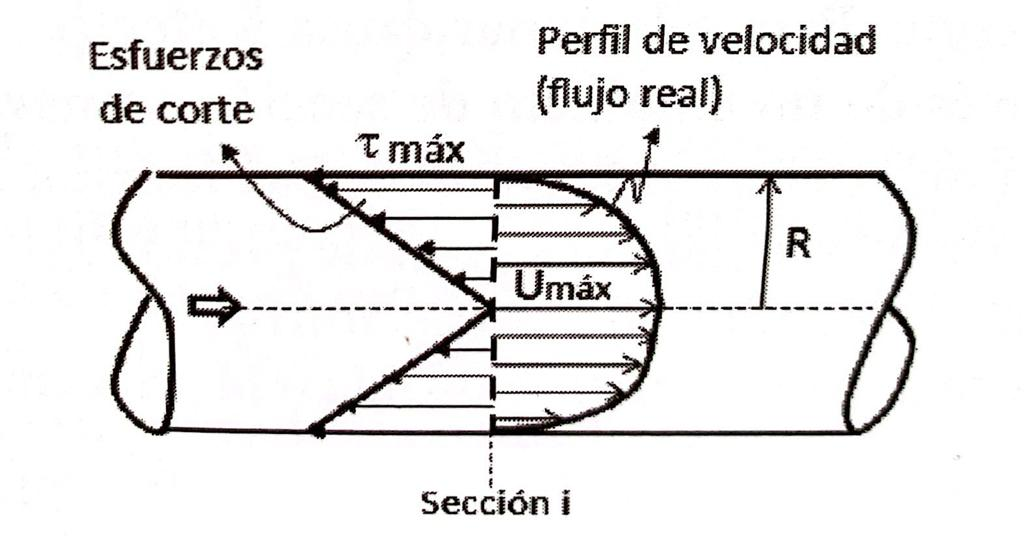
\includegraphics[width=8cm]{taun.jpeg}
\caption{Perfil de velocidades y esfuerzos de corte (tomado de \cite{agudelo2011mecanica}).}
\label{taun}
\end{figure}


% Ej 7.6 Street and Vennard
\begin{shaded}
\begin{exa}
Agua fluye en un conducto rectangular de secci\'on 0.9 m de ancho por 0.6 m de alto. La p\'erdida de cabeza de energ\'ia en este conducto de 60 m de longitud fue determinada experimentalmente e igual 10 m. a) Calcular el esfuerzo de corte en las paredes del conducto. Si el conducto es de secci\'on circular de di\'ametro $D = 0.6$m, b) ¿cual es el esfuerzo cortante en las paredes? y c) ¿dentro del flujo en un punto a 200 mm de las paredes?
\end{exa}
\end{shaded}

%%%%%%%%
\section{Experimentos de Reynolds} % From Shames
Osborne Reynolds en 1883 mediante un experimento el cual consisti\'o en establecer un flujo de agua a trav\'es de una tuber\'ia de vidrio en el que la velocidad era controlada por una valvula a la salida de la tuber\'ia (ver figura~\ref{reyn}). A la entrada de la tube\'ia se inyecta una tinta que tiene un peso espec\'ifico igual al del agua. Reynolds encontr\'o que cuando la v\'alvula est\'a ligeramente abierta, las part\'iculas de tinta se mueven de forma ordenada formando un filamento y a manera de capas que se deslizan una sobre otra sin mezclarse. Sin embargo, a medida que la v\'alvula se va abriendo, se alcanza una condici\'on en la cual la tinta presenta un movimiento fluctuante a medida que avanza en la tuber\'ia, en donde las part\'iculas de la tinta se mueven ca\'oticamente mezclandose. Al primer tipo de flujo se le llamo \emph{laminar} y al segundo \emph{turbulento}.

% FIg 9.2 from Shames 
\begin{figure}[h]
\centering
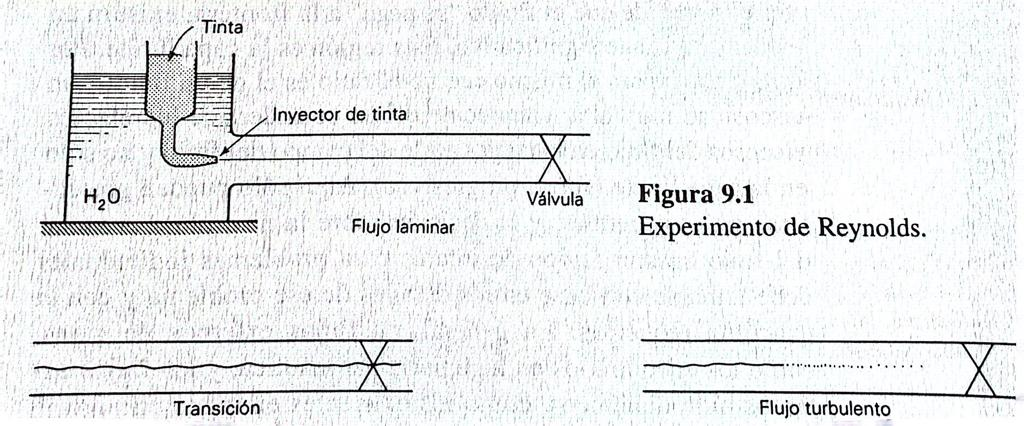
\includegraphics[width=8cm]{reyn.jpeg}
\caption{Experimento de Reynolds (tomado de \cite{irving2010fluid}).}
\label{reyn}
\end{figure}

% FIg 9.4 y 9.5 from Shames 
\begin{figure}[h]
\centering
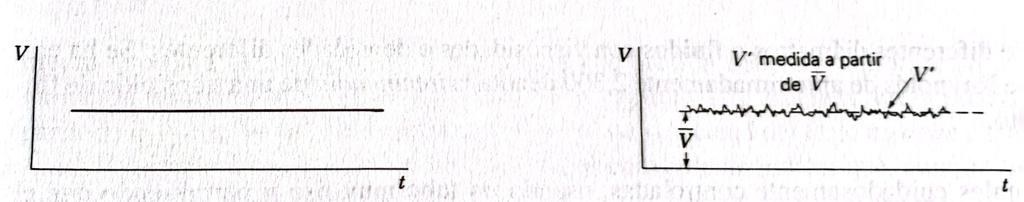
\includegraphics[width=8cm]{reyn1.jpeg}
\caption{Velocidad para flujo laminar y flujo turbulento (tomado de \cite{irving2010fluid}).}
\label{reyn1}
\end{figure}

Reynolds encontr\'o que el comportamiento de flujo se pod\'ia correlacionar con un parametro adimensional que relacionaba las fuerzas de inercia y las fuerzas viscosas, el cual es conocido como el \emph{numero de Reynolds (Re)}:

\begin{equation}
\color{red}\boxed{\color{black} Re = \frac{VD}{\nu} = \frac{1.273Q}{\nu D} }
\label{rey}
\end{equation}

donde $D$ es el di\'ametro de la tuber\'ia. 

Reynolds encontr\'o que flujo laminar se obten\'ia para valores de $Re<12000$, mientras que el flujo turbulento se lograba con $Re>50000$. Sin embargo estos valores encontrados por Reynolds se obtuvieron para condiciones alejadas de lo que es un sistema de conducci\'on real y que ocurren comunmente en ingenier\'ia. Para propositos pr\'acticos en tuber\'ias comerciales se ha encontrado que:
$$
Re < 2100 \rightarrow \text{flujo laminar}
$$
$$
2100 < Re < 4000 \rightarrow \text{flujo de transici\'on}
$$
$$
Re > 4000 \rightarrow \text{flujo de turbulento}
$$ 

%%%%%%%%
\section{Flujo laminar} % From Streeter
Se analiza primero el caso general de flujo permanente e incompresible entre placas paralelas e inclinadas a un angulo $\theta$, en donde la placa superior se mueve con una velocidad constante $U$ (ver figura~\ref{lami}) y la velocidad del flujo es $u=f(y)$. Si analizamos las fuerzas actuantes sobre el elemento diferencial de fluido de ancho unitario, espesor $\delta y$ y longitud $\delta l$ de la figura~\ref{lami}, tenemos:

% FIg 5.3 Streeter 
\begin{figure}[h]
\centering
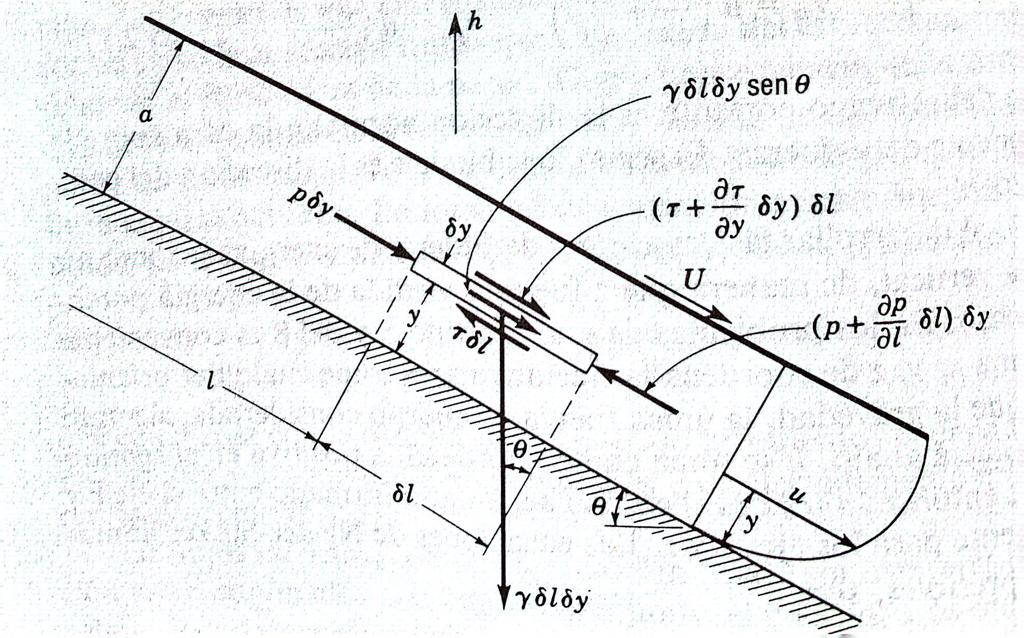
\includegraphics[width=8cm]{lami.jpeg}
\caption{Flujo en movimiento entre placas paralelas con placa superior en movimiento (tomado de \cite{streeter}).}
\label{lami}
\end{figure}

\begin{equation}
p \delta y - \left( p \delta y + \frac{\partial p}{\partial l} \delta l \delta y \right)- \tau \delta l + \left( \tau \delta l + \frac{\partial \tau}{\partial y} \delta y \delta l \right) + \gamma \delta l \delta y \sin \theta = 0
\label{lam1}
\end{equation}

donde $p$ es la presi\'on, $\gamma$ es el peso espec\'ifico del fluido y $\tau$ es el esfuerzo de corte. Simplificando la ecuaci\'on~\ref{lam1}, dividiendo por el diferencial de volumen $\delta l \delta y$ y reemplazando $\sin \theta = -\frac{\partial h}{\partial l}$, se tiene:

\begin{equation}
\frac{\partial \tau}{\partial y} = \frac{\partial}{\partial l} (p + \gamma h)
\label{lam2}
\end{equation}

donde $h$ es una distancia vertical positiva. Teniendo en cuenta que $u$ y por lo tanto $\tau$ varian con respecto a $y$ \'unicamente, $\frac{\partial \tau}{\partial y} = \frac{d \tau}{dy}$. De manera similar, si $(p + \gamma h)$ no cambia en $y$ (no hay aceleracion en $y$), esta cambia en direcci\'on de $l$, por lo tanto $\frac{\partial (p + \gamma h)}{\partial l} = \frac{d (p + \gamma h)}{dl}$. La ecuaci\'on queda:

\begin{equation}
\frac{d \tau}{dy} = \frac{d}{dl} (p + \gamma h)
\label{lam3}
\end{equation}

De la \emph{ley de viscosidad de Newton}, derivando $\tau$ con respecto a $y$, tenemos $\frac{d \tau}{dy} = \mu \frac{d^2 u}{dy^2}$, e igulando con la ecuacion~\ref{lam3}, se tiene:

\begin{equation}
\frac{d \tau}{dy} = \mu \frac{d^2 u}{dy^2} = \frac{d}{dl} (p + \gamma h)
\label{lam4}
\end{equation}

Integrando la ecuaci\'on~\ref{lam4} con respecto a $y$, se tiene:

\begin{equation}
\mu \frac{du}{dy} = y\frac{d}{dl} (p + \gamma h) + A 
\label{lam5}
\end{equation}

Inegrando la ecuaci\'on~\ref{lam5}, queda:

\begin{equation}
u = \frac{1}{2\mu} \frac{d}{dl} (p + \gamma h) y^2 + \frac{A}{\mu}y + B 
\label{lam6}
\end{equation}

donde $A$ y $B$ son constantes de integraci\'on. Si $u=0$ (velocidad en la placa fija) para $y=0$ y $u=U$ (velocidad de la placa movil) para $y=a$, las constantes pueden ser encontradas resultando que $B=0$ y que:

\begin{equation}
A = U\frac{\mu}{a} - \frac{a}{2}\frac{d}{dl} (p + \gamma h)
\label{lam7}
\end{equation}

Reemplazando las constantes en la ecuaci\'on~\ref{lam6}:

\begin{equation}
\color{red}\boxed{\color{black} u = \frac{Uy}{a}-\frac{1}{2\mu}\frac{d}{dl}(p + \gamma h)( ay - y^2 ) }
\label{lam8}
\end{equation}

Para el caso de placas horizontales, el gradiente debido a la presi\'on o altura es constante $p+ \gamma h = C$, por lo que, de la ecuaci\'on~\ref{lam8}, la distribucion de velocidades es $u = \frac{Uy}{a}$ (lineal). Para el caso en el que la placa superior es fija ($U=0$), $u = -\frac{1}{2\mu}\frac{d}{dl}(p + \gamma h)( ay - y^2 )$. Notese que la velocidad maxima es cuando $y = \frac{a}{2} - \frac{\mu U}{a \frac{d}{dl}(p + \gamma h)}$. 

El caudal ($Q$) que pasa a trav\'es de una secci\'on transversal, se obtiene como:

\begin{equation}
Q = \int_0^a u dy = \left( U\frac{y^2}{2a} - \frac{1}{4\mu}\frac{d}{dl}(p+ \gamma h) y^2 a + \frac{1}{6\mu}\frac{d}{dl}(p+ \gamma h) y^3 \right) \bigg|_0^a = \frac{Ua}{2} - \frac{1}{12\mu}\frac{d}{dl}(p + \gamma h)a^3
\label{lam8}
\end{equation}

%\subsection{Perdidas en flujo laminar}
\subsection{Flujo laminar en conductos y coronas} % From Streeter
Supongamos que consideramos una tuber\'ia circular inclinada con flujo permanente (ver figura~\ref{lamt}). Si se toma un anillo de flujo de espesor infinitesimal $\delta r$, las fuerzas actuantes en la direcci\'on de flujo son:

% FIg 5.3 Streeter 
\begin{figure}[h]
\centering
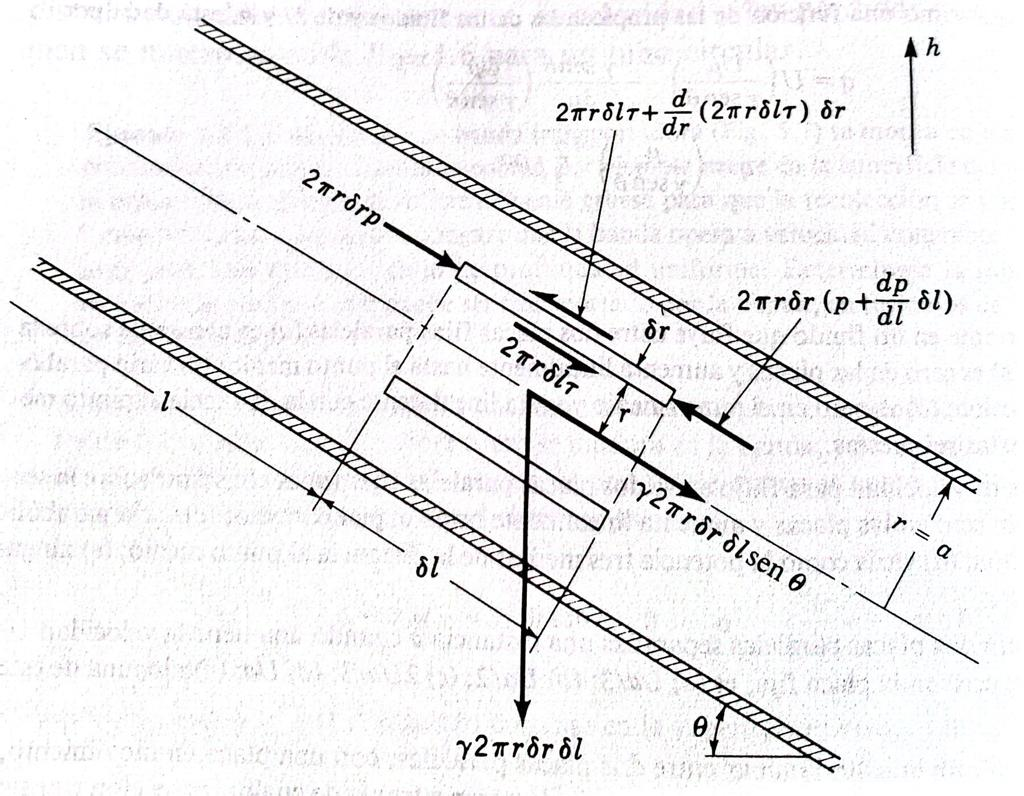
\includegraphics[width=8cm]{lamt.jpeg}
\caption{Diagrama de cuerpo de libre de un elemento cili\'ndrico para flujo laminar en un tubo circular inclinado (tomado de \cite{streeter}).}
\label{lamt}
\end{figure}

\begin{equation}
2\pi r \delta r p -\left( 2\pi r \delta r p + 2\pi r \delta r \frac{dp}{dl} \delta l \right ) + 2\pi r \delta l \tau - \left[ 2\pi r \delta l \tau + \frac{d}{dr}(2\pi r \delta l \tau) \delta r \right] + \gamma 2 \pi r \delta r \delta l \sin \theta = 0  
\label{lam9}
\end{equation}

Teniendo en cuenta que $\sin \theta = -\frac{dh}{dl}$ y simplificando  la ecuaci\'on~\ref{lam9}, se tiene:

\begin{equation}
- 2\pi r \delta r \frac{dp}{dl} \delta l  - \frac{d}{dr}(2\pi r \delta l \tau) \delta r  - \gamma 2 \pi r \delta r \delta l \frac{dh}{dl} = 0  
\label{lam10}
\end{equation}

dividiendo por el volumen del anillo $2\pi r\delta r \delta l$, se tiene que:

\begin{equation}
\frac{d}{dl}(p + \gamma h) + \frac{1}{r}\frac{d}{dr}(\tau r) = 0
\label{lam11}
\end{equation}

Teniendo en cuenta que $d(p + \gamma h)/dl$ no es una funci\'on de $r$ y separando t\'erminos en la ecuaci\'on~\ref{lam11} para integrar con respecto a $r$:

\begin{equation}
\frac{d}{dl}(p + \gamma h) r dr + d(\tau r ) = 0
\label{lam12}
\end{equation}

Integrando la ecuaci\'on~\ref{lam12}, tenemos:
 
\begin{equation}
\frac{r^2}{2}\frac{d}{dl}(p + \gamma h) + \tau r = A
\label{lam13}
\end{equation}

donde $A$ es una constante de integraci\'on. De la ley de viscosidad de Newton, $\tau = - \mu \frac{du}{dr}$, reemplazando en la ecuaci\'on~\ref{lam13} tenemos:

\begin{equation}
\frac{r^2}{2}\frac{d}{dl}(p + \gamma h) -\mu \frac{du}{dr} r = A
\label{lam14}
\end{equation}

Separando t\'erminos para integraci\'on en la ecuaci\'on~\ref{lam14}, se tiene:

\begin{equation}
du = \frac{1}{2\mu} \frac{d}{dl}(p + \gamma h) r dr -\frac{A}{\mu}\frac{dr}{r}
\label{lam15}
\end{equation}
 
integrando la ecuaci\'on~\ref{lam15}, tenemos:

\begin{equation}
u = \frac{r^2}{4\mu}\frac{d}{dl}(p + \gamma h) - \frac{A}{\mu} \ln r + B 
\label{lam16}
\end{equation}

donde $B$ es una constante de integraci\'on. Si se tiene una corona circular como la que se muestra en la figura~\ref{lamc}, en donde la velocidad para el radio interior $r=b$ es $u=0$ y donde la velocidad para el radio exterior $r=a$ es $u=0$, las constantes de integraci\'on $A$ y $B$ en la ecuaci\'on~\ref{lam16} quedar\'ian:

% Fig 5.9 Streeter 
\begin{figure}[h]
\centering
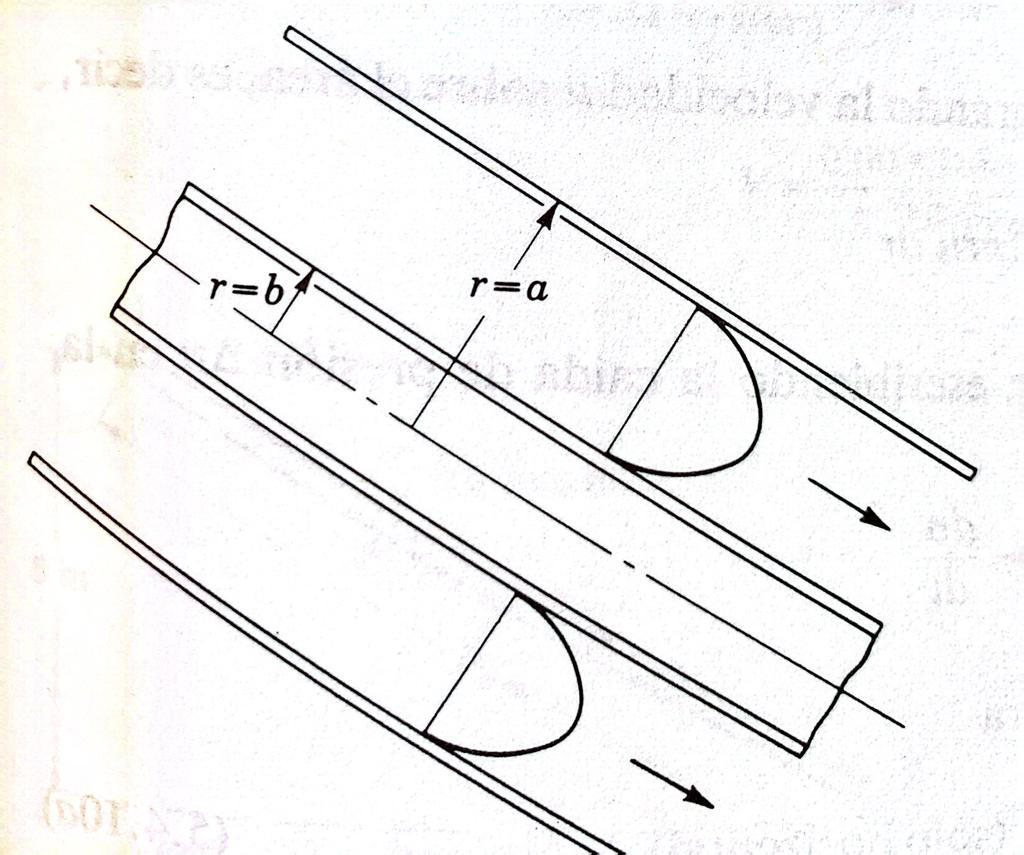
\includegraphics[width=8cm]{lamc.jpeg}
\caption{Flujo a trav\'es de un cilindro concentrico (tomado de \cite{streeter}).}
\label{lamc}
\end{figure}

\begin{equation}
B = \frac{A}{\mu}\ln a - \frac{a^2}{4\mu}\frac{d}{dl}(p + \gamma h)
\label{lam17}
\end{equation}

\begin{equation}
A = \frac{1}{4\ln(a/b)} \frac{d}{dl}(p + \gamma h) (a^2 - b^2)
\label{lam18}
\end{equation}

Reemplazando las constantes en la ecuaci\'on~\ref{lam16}, se tiene una expresi\'on para el perfil de velocidades en una corona circular:

\begin{equation}
\color{red}\boxed{\color{black} u = -\frac{1}{4\mu}\frac{d}{dl}(p + \gamma h) \left[ a^2 - r^2 + \frac{a^2 - b^2}{\ln(b/a)} \ln \frac{a}{r} \right ]}
\label{lam19}
\end{equation}

El caudal $Q$ se calcula como:

\begin{equation}
\begin{split}
Q & = \int_b^a 2\pi r u dr = \int_b^a -\frac{\pi r}{2\mu}\frac{d}{dl}(p + \gamma h) \left[  a^2 - r^2 + \frac{a^2 - b^2}{\ln(b/a)} \ln \frac{a}{r} \right ] dr \\
& = -\frac{\pi}{2\mu}\frac{d}{dl}(p + \gamma h)\int_b^a \left[ r a^2 - r^3 + \frac{(a^2 - b^2 )r}{\ln(b/a)}\ln \frac{a}{r} \right]dr \\
& = -\frac{\pi}{2\mu}\frac{d}{dl}(p + \gamma h)\int_b^a \left[ r a^2 - r^3 + \frac{(a^2 - b^2 )}{\ln(b/a)}(r\ln a - r ln r) \right]dr 
\end{split}
\label{lam20}
\end{equation}

Integrando la ecuaci\'on~\ref{lam20} y simplificando, se tiene:

\begin{equation}
\color{red}\boxed{\color{black} Q = -\frac{\pi}{8\mu}\frac{d}{dl}(p + \gamma h) \left[ a^4 - b^4 - \frac{(a^2 - b^2)^2 }{\ln (a/b)} \right]  }
\label{lam21}
\end{equation}

\subsection{Flujo laminar en tuber\'ias circulares: ecuaci\'on de Hagen-Poiseuille} % From Streeter
En un tubo circular, en la ecuacion\'on~\ref{lam14},  $A=0$ cuando $r=0$. Por lo tanto, la ecuaci\'on~\ref{lam16} queda:

\begin{equation}
u = \frac{r^2}{4\mu}\frac{d}{dl}(p + \gamma h) + B 
\label{lam22}
\end{equation}

Si $u=0$ cuando $r=a$, se tiene que $B=-\frac{a^2}{4\mu}\frac{d}{dl}(p + \gamma h)$, reemplazando en la ecuaci\'on~\ref{lam22}, se tiene:

\begin{equation}
\color{red}\boxed{\color{black} u = \frac{r^2 - a^2}{4\mu}\frac{d}{dl}(p + \gamma h) }
\label{lam23}
\end{equation}

La ecuaci\'on~\ref{lam23} representa la distribuci\'on de velocidades en una tuber\'ia circular, cuya forma es un paraboloide de revoluci\'on (ver figura~\ref{lamc1}). 

% Fig 5.6 Streeter 
\begin{figure}[h]
\centering
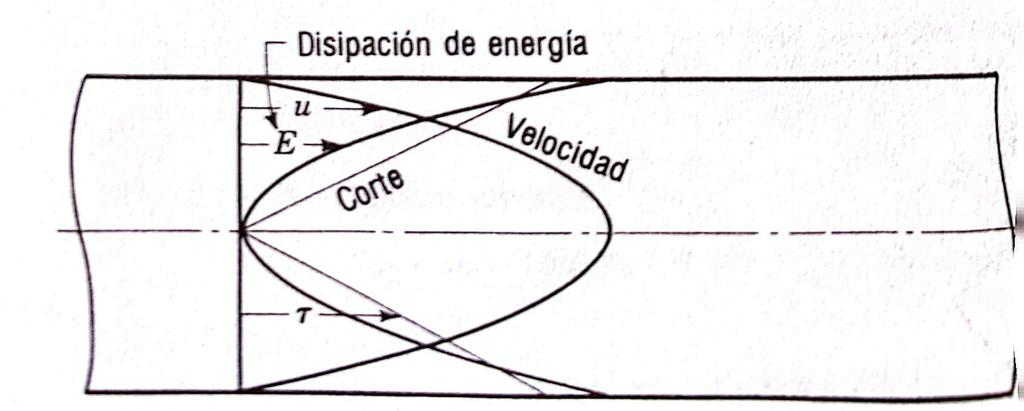
\includegraphics[width=8cm]{lamc1.jpeg}
\caption{Distribuci\'on de velocidades y esfuerzos de corte en una tuber\'ia circular (tomado de \cite{streeter}).}
\label{lamc1}
\end{figure}

La velocidad m\'axima $u_{max}$ ocurre cuando $r=0$, por lo tanto de la ecuaci\'on~\ref{lam23} se tiene:

\begin{equation}
\color{red}\boxed{\color{black} u_{max} = -\frac{a^2}{4\mu}\frac{d}{dl}(p + \gamma h) }
\label{lam24}
\end{equation}

El caudal $Q$ se calcula como:

\begin{equation}
 Q = \int_0^a 2\pi r u dr = \frac{\pi}{2\mu}\frac{d}{dl}(p + \gamma h) \int_0^a (r^3 -r a^2) dr 
\label{lam25}
\end{equation}

Integrando la ecuaci\'on~\ref{lam25}

\begin{equation}
\color{red}\boxed{\color{black} Q =  -\frac{\pi a^4}{8\mu}\frac{d}{dl}(p + \gamma h) }
\label{lam26}
\end{equation}

La \emph{velocidad media} se define como $V = \frac{Q}{V} = \frac{Q}{\pi a^2}$, que ademas es la mitad del paraboloide de revoluci\'on de velocidades (mitad de la velocidad m\'axima), de acuerdo con esto:
 
\begin{equation}
\color{red}\boxed{\color{black} V = -\frac{a^2}{8\mu}\frac{d}{dl}(p + \gamma h) }
\label{lam27}
\end{equation}

Para un tubo horizontal de longitud $L$, $h$ es constante, por lo tanto:

\begin{equation}
\frac{\Delta p}{L} = -\frac{dp}{dl}
\label{lam28}
\end{equation}

donde $\Delta p$ es la ca\'ida de presi\'on a lo largo de $L$. Para el caso de un tubo horizontal, $Q$ se expresa en t\'erminos del di\'ametro $D$ como:

\begin{equation}
\color{red}\boxed{\color{black} Q = \frac{\Delta p \pi D^4}{128 \mu L} }
\label{lam29}
\end{equation}

La ecuaci\'on anterior es conocida como la \emph{ecuaci\'on de Hagen-Poiseuille}. La velocidad media a partir de la ecuaci\'on~\ref{lam29}:

\begin{equation}
\color{red}\boxed{\color{black} V = \frac{\Delta p D^2}{32 \mu L} }
\label{lam30}
\end{equation}

% Ej 5.3 Streeter 
\begin{shaded}
\begin{exa}
Determinese la direcci\'on de flujo del tubo mostrado en la figura en donde $\gamma = 8000$ N/ m$^2$ y $\mu = 0.04$ kg/m.s. Adem\'as, encontrar el caudal en litros por segundo y el n\'umero de Froude.
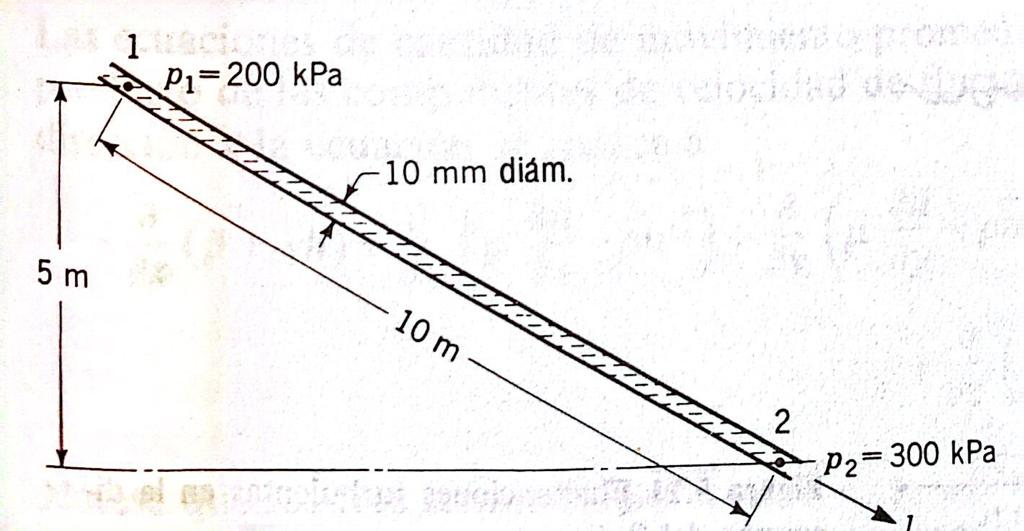
\includegraphics[width=8cm]{exa1.jpeg}
\end{exa}
\end{shaded}

De la ecuaci\'on~\ref{lam29}, despejando la ca\'ida de presi\'on $\Delta p$ para una tuber\'ia horizontal, la cual representa las \emph{p\'erdidas por unidad de volumen} $h_e$, se tiene:

\begin{equation}
\color{red}\boxed{\color{black} \Delta p = h_e = \frac{128 \mu LQ}{\pi D^4} }
\label{lam311}
\end{equation}

El \emph{factor de correcci\'on de la energ\'ia cin\'etica} $\alpha$ para flujo laminar en una tuber\'ia se calcula como:

\begin{equation}
\alpha = \frac{1}{A} \int \left ( \frac{u}{V} \right )^3 dA
\label{lam31}
\end{equation}

Reemplazando las ecuaciones~\ref{lam23} y ~\ref{lam27} en la ecuaci\'on~\ref{lam31}, tenemos:

\begin{equation}
\alpha = \frac{1}{\pi a^2} \int_0^a \left\{ 2 \left[ 1- \left(\frac{r}{a}\right)^2 \right] \right\}^3 2\pi r dr = 2
\label{lam32}
\end{equation}

Notese que la energ\'ia cin\'etica es el doble de la energ\'ia si se considera una distribuci\'on uniforme de velocidades. El \emph{factor de correcc\'ion de la cantidad de movimiento} $\beta$, se expresa como:

\begin{equation}
\beta = \frac{1}{A} \int \left ( \frac{u}{V} \right )^2 dA
\label{lam33}
\end{equation}

Reemplazando las ecuaciones~\ref{lam23} y ~\ref{lam27} en la ecuaci\'on~\ref{lam33}, tenemos que $\beta = 4/3$.

\section{Flujo turbulento}
\subsection{Esfuerzo de corte turbulento} % From Streeter
En un flujo turbulento, las part\'iculas de agua viajan de manera desordenada siguiente trayectorias ca\'oticas. Esto implica que las velocidades y las presiones fluctuen r\'apidamente en el tiempo. Esto implica que el an\'alisis de las ecuaciones de Navier-Stokes sea dificil anal\'iticamente, e incluso, num\'ericamente. Para esto es necesario expresar dichas cantidades en sus valores medios en el tiempo y en sus cantidades fluctuantes. Para la componente de la velocidad en $x$, $u$, esta se puede representar:

% Fig 5.11 Streeter 
\begin{figure}[h]
\centering
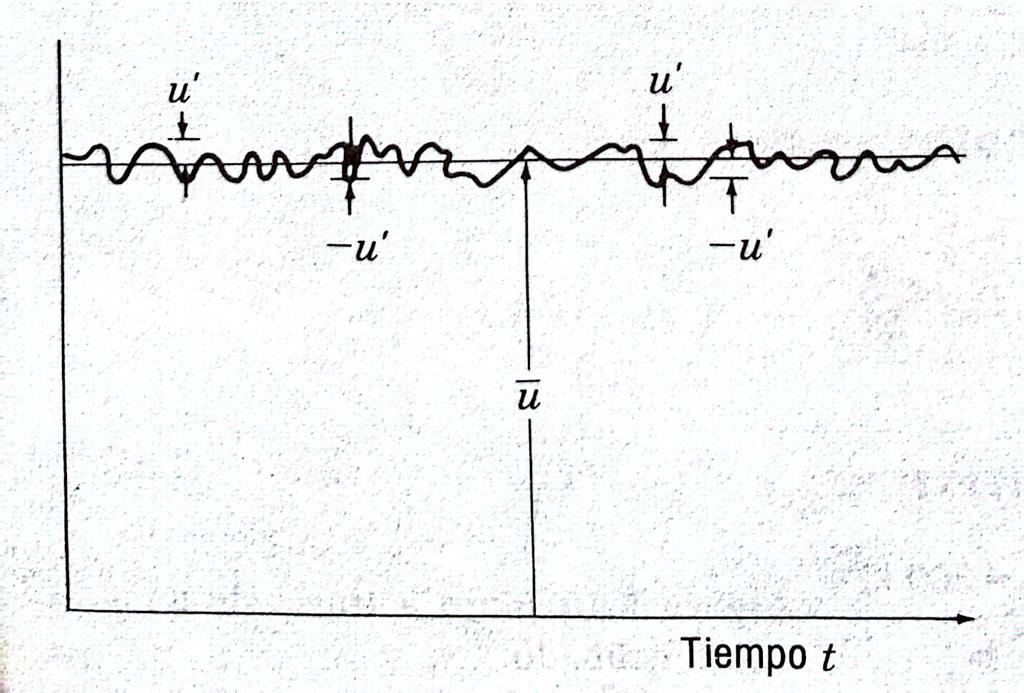
\includegraphics[width=8cm]{turb.jpeg}
\caption{Velocidad en $x$ para flujo turbulento (tomado de \cite{streeter}).}
\label{turb}
\end{figure}


\begin{equation}
u = \overline{u} + u'
\label{tur1}
\end{equation}

donde $\overline{u}$ es la velocidad media o promedio y $u'$ es la fluctuaci\'on. Para un tiempo $T$, $\overline{u}$ se expresa:

\begin{equation}
\overline{u} = \frac{1}{T} \int_0^T u dt
\label{tur2}
\end{equation}

y el promedio de las fluctuaciones de $u$ en $T$, se expresa como:

\begin{equation}
\overline{u'} = \frac{1}{T} \int_0^T (u-\overline{u}) dt = 0
\label{tur3}
\end{equation}

N\'otese que el promedio de $u'$ es cero para $T$. Sin embargo el cuadrado de las fluctuaciones:

\begin{equation}
\overline{{u'}^2} = \frac{1}{T} \int_0^T (u-\overline{u})^2 dt \neq 0
\label{tur4}
\end{equation}
 
es diferente de cero. Reynolds descompuso cada propiedad del flujo en su valor medio y su fluctuaci\'on:

\begin{equation}
v = \overline{v} + v' \hspace{2cm} w = \overline{w} + w' \hspace{2cm} p = \overline{p} + p'
\label{tur44}
\end{equation}

Note que la raiz cuadrada de $\overline{{u'}^2}$  es una medida de la \emph{intensidad de la turbulencia}. Tampoco es cero los productos medios de las fluctuaciones como $\overline{u' v'}$, $\overline{u' w'}$, etc.

De las ecuaciones de Navier-Stokes (ecuaciones~\ref{nast1}, ~\ref{nast2} y ~\ref{nast3}), la ecuaci\'on de cantidad de movimiento en $x$ promediada en el tiempo, la cual contiene el producto de las componentes de fluctuaci\'on, se expresa como:

\begin{equation}
-\frac{\partial}{\partial x}(\overline{p} + \gamma h) + \frac{\partial}{\partial x}\left( \mu \frac{\partial \overline{u}}{\partial x} - \rho \overline{{u'}^2} \right) + \frac{\partial}{\partial y}\left( \mu \frac{\partial \overline{u}}{\partial y} - \rho \overline{u' v'} \right) + \frac{\partial}{\partial z}\left( \mu \frac{\partial \overline{u}}{\partial z} - \rho \overline{u' w'} \right) = \rho \frac{\partial \overline{u}}{\partial t}
\label{tur5}
\end{equation}

Los t\'erminos $-\rho \overline{{u'}^2}$, $-\rho \overline{u' v'}$ y $-\rho \overline{u' w'}$, representan la aceleraci\'on convectiva y matem\'aticamente son an\'alogos al esfuerzo. Estos se denominan los \emph{esfuerzos de Reynolds}. Note que los t\'erminos (e.g. $\mu\frac{\partial \overline{u}}{\partial x}$) son los esfuerzos cortantes medios viscosos. Los esfuerzos de Reynolds son los responsables del intercambio de cantidad de movimiento y la capacidad de mezcla en un flujo turbulento. En un flujo turbulento los esfuerzos de Reynolds son superiores a los esfuerzos viscosos, mas aun, en la capa l\'imite. Los esfuerzos de Reynolds se calculan empiricamente con ayuda de experimentos. 

Para flujo en la direcci\'on $x$, el esfuerzo turbulento mas importante es $-\rho \overline{u' v'}$, por lo que la ecuaci\'on~\ref{tur5} se convierte:
 \begin{equation}
-\frac{\partial}{\partial x}(\overline{p} + \gamma h) + \frac{\partial \tau}{\partial y} \approx \rho \frac{\partial \overline{u}}{\partial t}
\label{tur6}
\end{equation}

donde $\tau = \tau_l + \tau_t = \mu \frac{\partial \overline{u}}{\partial y} - \rho \overline{u' v'}$ es el esfuerzo de corte total, $\tau_l$ es el eufuerzo laminar y $\tau_t$ es el esfuerzo turbulento. 

\subsection{Longitud de mezcla de Prandtl} % From Streeter
El esfuerzo cortante aparente para flujo turbulento, incluyendo los efectos viscosos, se expresa como:

\begin{equation}
\tau = (\mu + \eta) \frac{du}{dy}
\label{tur60}
\end{equation}


Prandtl encontr\'o expresiones para determinar $u'$ y $v'$ en funci\'on de la \emph{longitud de mezcla} $l$ y el gradiente de velocidad $\frac{du}{dy}$ en donde $u$ es la velocidad media temporal en un punto y $y$ es la distancia normal a $u$ medida desde la frontera (ver figura~\ref{mez})

% Fig 5.12 Streeter 
\begin{figure}[h]
\centering
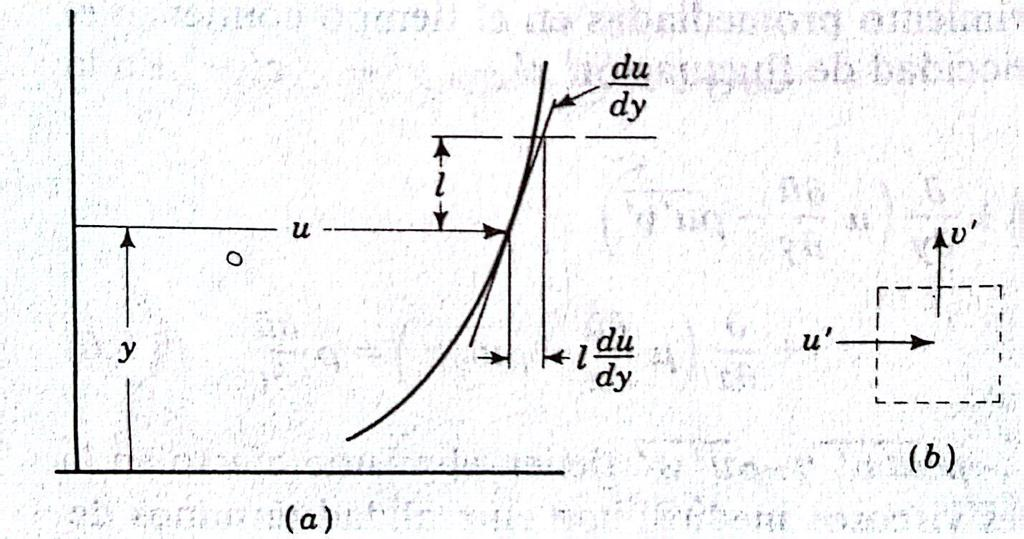
\includegraphics[width=8cm]{mez.jpeg}
\caption{Esquema de la teor\'ia de longitud de mezcla (tomado de \cite{streeter}).}
\label{mez}
\end{figure}

De la figura~\ref{mez}, $l$ y $u'$ se relacionan como:

\begin{equation}
u' \sim l \frac{du}{dy}
\label{tur8}
\end{equation}

Esto significa que los cambios de la magnitud de la velocidad dependen de los cambios en la velocidad media temporal en dos punto separados por $l$, donde $l$  es el taman\~no promedio de los remolinos responsables de la mezcla. Teniendo en cuenta que $u'$ y $v'$ est\'an correlacionados:

\begin{equation}
v' \sim u' \sim l \frac{du}{dy}
\label{tur9}
\end{equation}

Reemplazando las expresiones de la ecuaci\'on~ref{tur9} en $\tau_t = -\rho \overline{u' v'}$ (esfuerzo turbulento), se obtiene una ecuaci\'on que define la longitud de mezcla $l$:

\begin{equation}
\tau_t = \rho l^2 \left( \frac{du}{dl} \right)^2
\label{tur10}
\end{equation}

Note que $l$ absorbe el factor de proporcionalidad y el signo. 

Para flujo turbulento, se puede encontrar una expresi\'on similar a la ley de viscosidad de Newton como:

\begin{equation}
\tau_t = \eta\frac{du}{dy}
\label{tur11}
\end{equation}

donde $\eta$ es la \emph{viscosidad de remolino} que no es solo una propiedad del fluido ya que depende del movimiento de este y de su densidad, y generalmente es mayor $\mu$. $\eta$ tambi\'en se considera como un coeficiente de transferencia de cantidad de movimiento. Igualando las ecuaciones~\ref{tur10} y ~\ref{tur11}, se tiene:

\begin{equation}
\eta=\rho l^2 \frac{du}{dy}
\label{tur12}
\end{equation}

Note que $l$ cambia con respecto a la distancia a la pared $y$ y se hace cero en la frontera. Von Karman a trav\'es del estudio de relaciones de similitud en flujo turbulento, encontr\'o una relaci\'on para $l$ como:

\begin{equation}
l= \kappa \frac{du/dy}{d^2 u / dy^2}
\label{tur13}
\end{equation}

donde $\kappa$ es una constante universal (\emph{constante de Von Karman}) en un flujo turbulento sin importar la configuraci\'on de la frontera o el n\'umero de Reynolds. Se ha encontrado que $\kappa \approx 0.40$.

\subsection{Distribuciones de velocidad} % From Streeter
En flujos de turbulentos, la distribuci\'on de velocidades en las zonas cercanas a la pared del conducto se puede dividir en tres capas (ver Figura~\ref{distr}): \emph{Capa viscosa (o laminar)}, \emph{capa de traslape} y \emph{zona turbulenta exterior}. 

% Fig 5.13 Streeter 
\begin{figure}[h]
\centering
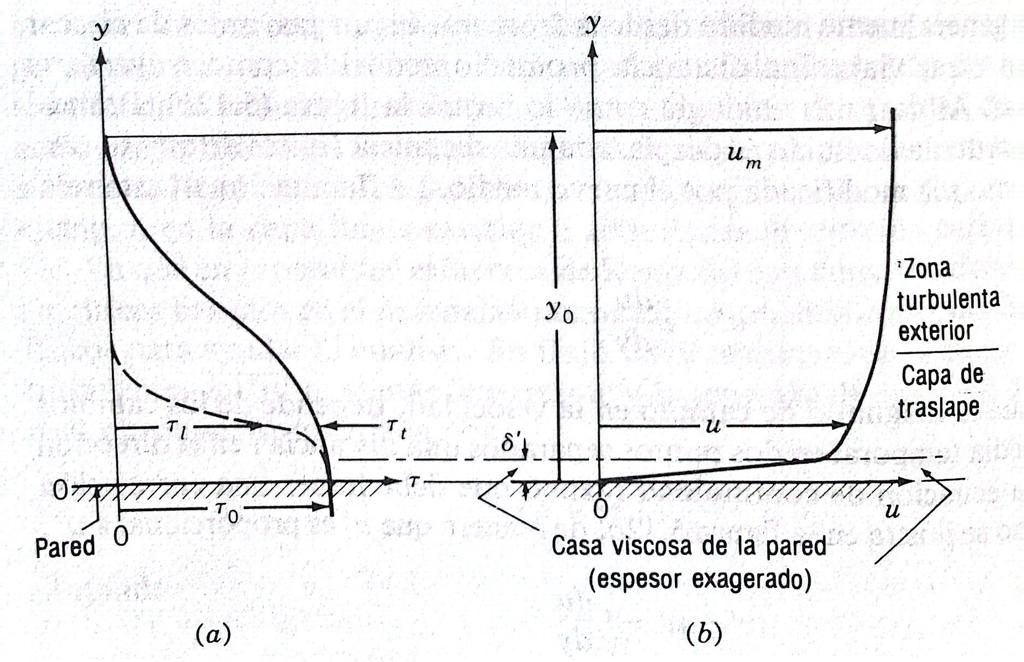
\includegraphics[width=8cm]{distr.jpeg}
\caption{Para flujo turbulento en conductos a) distribuci\'on de esfuerzos y b) distribuci\'on de velocidades (tomado de \cite{streeter}).}
\label{distr}
\end{figure}


\subsubsection*{Capa laminar} % From Streeter
En la capa viscosa mas cercana a la pared, el esfuerzo cortante es constante e igual al esfuerzo en la pared $\tau_0$. La distribuci\'on de velocidades en la capa viscosa se relaciona con la viscosidad absoluta y el esfuerzo cortante a partir de la ley de viscosidad de Newton  y se expresa como:

\begin{equation}
\frac{\tau_0 }{\rho} = \frac{\mu}{\rho}\frac{u}{y} = \nu \frac{u}{y} \hspace{2cm} y \leq \delta'
\label{dist1}
\end{equation}

donde $\delta '$ es el espesor de la capa viscosa de la pared.

Definiendo la \emph{velocidad de esfuerzo de corte} ($u^*$) como $u^*=\sqrt{\tau_0 / \rho}$ y reemplazando en la ecuaci\'on~\ref{dist1}, se tiene:

\begin{equation}
{u^* }^2 = \nu \frac{u}{y}
\label{dist2}
\end{equation}

multiplicando por $u$ e invirtiendo los t\'erminos en la ecuaci\'on~\ref{dist2}, se tiene

\begin{equation}
\color{red}\boxed{\color{black} \frac{u}{u^*} = \frac{u^* y}{\nu} } \hspace{2cm} \color{black} y \leq \delta' 
\label{dist3}
\end{equation}

La ecuaci\'on~\ref{dist3} muestra una relaci\'on lineal entre $u$ y $y$ en la capa viscosa (o laminar) y es conocida como la \emph{ley de pared}. A trav\'es de experimentos, se ha encontrado que $\delta '$:

\begin{equation}
\color{red}\boxed{\color{black} \delta ' = 5 \frac{\nu}{u^* } }
\label{dist4}
\end{equation}

En la practica, se ha encontrado que una superficie es hidr\'aulicamente lisa si $\delta ' > 6 \varepsilon$ e hidr\'aulicamente rugosa si $\delta ' < 3 \varepsilon$, donde $\varepsilon$ es la rugosidad en unidades de $L$ del material del conducto.

\subsubsection*{Capa de traslape} % From Streeter
En la capa de traslape (ver figura~\ref{distr}),  los esfuerzos turbulentos son dominantes mientras que el esfuerzo laminar puede ser despreciable. Por lo tanto el esfuerzo cortante turbulento  $\tau_t$ (Ecuaci\'on~\ref{tur10}) es aproximadamente igual al esfuerzo cortante en la pared $\tau_0$

\begin{equation}
\tau_0 = \rho l^2 \left( \frac{du}{dy} \right)^2
\label{dist5}
\end{equation}

Von Karman encontr\'o que la longitud de mezcla $l$ en cercan\'ia a la pared es proporcional a la distancia desde la pared $y$ e igual $l \approx \kappa y$. Reemplazando $l$  y $u^*$ en la ecuaci\'on~\ref{dist4}, se tiene que:

\begin{equation}
\frac{du}{u^*} = \frac{1}{\kappa} \frac{dy}{y}
\label{dist6}
\end{equation}

integrando la ecuaci\'on~\ref{dist6}:

\begin{equation}
\frac{u}{u^*} = \frac{1}{\kappa} \ln y + A
\label{dist7}
\end{equation}

donde $A$ es una constante de integraci\'on. Si se reemplaza la expresi\'on para $u$ de la ecuaci\'on~\ref{dist7} en la ecuaci\'on~\ref{tur13}, se tiene que $l$ es proporcional a $y$ (note que $\frac{d^2 u}{dy^2}$ es negativo por que el gradiente de velocidad disminuye en la medida que $y$ aumenta). 

Para $y = \delta '$ se tiene que $u= u_w$ que es la velocidad en donde el flujo cambia de laminar a turbulento. Reemplazando en la ecuaci\'on~\ref{dist3}, se tiene:

\begin{equation}
\frac{u_w}{u^*} = \frac{u^* \delta '}{\nu} = N
\label{dist8}
\end{equation}

donde $N$ es un n\'umero de Reynolds cr\'itico cuando el flujo cambia de laminar a turbulento. Sustituyendo $u= u_w $ y $y = \delta '$ en la ecuaci\'on~\ref{dist7} para determinar el valor de $A$, se tiene que:

\begin{equation}
A = \frac{u_w }{u^* } - \frac{1}{\kappa} \ln \delta ' = N - \frac{1}{\kappa} \ln \left( \frac{N \nu}{u^*} \right) =N - \frac{1}{\kappa}  ( \ln N + \ln \nu  - \ln u^* )  
\label{dist9}
\end{equation}

Reemplazando la ecuaci\'on~\ref{dist9} en la ecuaci\'on~\ref{dist8}, se tiene:

\begin{equation}
\color{red}\boxed{\color{black} \frac{u}{u^*} = \frac{1}{\kappa} \ln \left(\frac{y u^*}{\nu}\right) + N - \frac{1}{\kappa} \ln N }
\label{dist10}
\end{equation}

Nikuradse mediante experimentos de flujo turbulento para conductos con paredes lisas y graficando $u/u^*$ vs $\ln(y u^*/ \nu )$ encontr\'o que la constante universal adimensional $\kappa = 0.40$ y  $N - \frac{1}{\kappa} \ln N  = 5.5$.

\subsubsection*{Zona turbulenta}
En la zona turbulenta de la figura~\ref{distr} para tuber\'ias de radio $r_0$ y reemplazando $y=r_0$, para el cual la velocidad $u=u_m $ (en el centro de la tuber\'ia), en la ecuaci\'on~\ref{dist7}, se tiene que la constante es:

\begin{equation}
A = \frac{u_m}{u^*} - \frac{1}{\kappa} \ln r_0
\label{dist11}
\end{equation}

Reemplazando en la ecuaci\'on~\ref{dist7}:

\begin{equation}
\color{red}\boxed{\color{black} \frac{u_m-u}{u^*} = \frac{1}{\kappa} \ln \frac{r_0}{y} }
\label{dist12}
\end{equation}

La ecuaci\'on~\ref{dist12} es conocida como la \emph{ley del deficit de velocidad} y se aplica a conductos lisos y rugosos.

Para tubos rugosos, $y_w = m \epsilon '$, donde $\epsilon '$ es una altura t\'ipica de la rugosidad y $m$ es un coeficiente de forma que depende de la naturaleza de la rugosidad, y la velocidad es $u_w$, determinando el valor de la constante en la ecuaci\'on~\ref{dist7}, se tiene:
 
\begin{equation}
A = \frac{u_m}{u^*} - \frac{1}{\kappa} (\ln m - \ln \epsilon ')
\label{dist13}
\end{equation}

reemplazando la ecuaci\'on~\ref{dist13} en la ecuaci\'on~\ref{dist7}, se tiene:

\begin{equation}
\color{red}\boxed{\color{black} \frac{u}{u^*} = \frac{1}{\kappa}\ln \frac{y}{\epsilon '} + \frac{u_w}{u^*}-\frac{1}{\kappa}\ln m }
\label{dist14}
\end{equation}

donde el termino $\frac{u_w}{u^*}-\frac{1}{\kappa}\ln m$ es una constante que depende del tipo de rugosidad. Nikuradse realizando experimentos con tuber\'ias rugosas (granos de arena aheridos a las paredes de la tuber\'ia) y considerando que la rugosidad de la tuber\'ia $\epsilon '$ es igual al di\'ametro del grano de arena, encontr\'o que $\kappa = 0.40$ y $\frac{u_w}{u^*}-\frac{1}{\kappa}\ln m =8.48$. 

Note que la \emph{ley logar\'itmica} de la ecuaci\'on~\ref{dist10} es la que tiene la aplicaci\'on mas amplia. F\'ijese que la capa viscosa es muy peque\~na en flujos turbulentos.

Prandtl desarroll\'o una formula sencilla para la distribuci\'on exponencial de velocidad para flujo turbulento en tuber\'ias:

\begin{equation}
\color{red}\boxed{\color{black} \frac{u}{u_m } = \left( \frac{y}{r_0} \right)^n  }
\label{dist15}
\end{equation}

donde $n$ varia con el n\'umero de Reynolds. Esta ecuaci\'on emp\'irica es valida solo para ciertas distancias de la pared. Para $R < 100000$, $n=1/7$, para valores mayores de $R$, $n$ decrece. Ambas ecuaciones ~\ref{dist15} y ~\ref{dist10} tienen la falla de predecir un valor $du/dy \neq 0$ en el centro de la tuber\'ia.

% Ej 5.5 Streeter
\begin{shaded}
\begin{exa}
Encuentrese una expresi\'on  aproximada para la distribuci\'on de longitud de mezclado en flujo turbulento en un tubo a partir de la ley exponencial de velocidad de Prandtl para $n=1/7$. 
\end{exa}
\end{shaded}

% Ej 5.5 Streeter
\begin{shaded}
\begin{exa}
En un tubo circular de 14 $cm$ di\'ametro fluye aire a una temperatura de $T = 20$ $^o$C. Si el flujo esta completamente desarrollado, y la velocidad en el centro de la tuber\'ia es 5 $m/s$, determinar a) la velocidad de fricci\'on $u^*$ y b) el esfuerzo de corte en la pared. Asumir flujo turbulento y la ocurrencia de la ley logar\'itmica.
\end{exa}
\end{shaded}

\subsection{P\'erdidas de energ\'ia} % From Streeter
En flujos incompresibles y turbulentos a regimen permanente y uniforme en conductos cerrados de secci\'on transversal constante, el esfuerzo cortante en la pared $\tau_0$ se expresa como:

\begin{equation}
\color{red}\boxed{\color{black} \tau_0 = \lambda \frac{\rho}{2} V^2 }
\label{perd0}
\end{equation}

donde $\lambda$ es un coeficiente  adimensional y $V$ es la velocidad media. En conductos abiertos o cerrados no circulares, el esfuerzo cortante no es constante sobre la superficie por lo que $\tau_0$ se calcula como el promedio de los esfuerzos cortantes sobre la pared. 

Si se analizan las fuerzas actuantes sobre un volumen de control de flujo en un conducto abierto o cerrado (ver figura~\ref{perd}), la energ\'ia del flujo podr\'ia proporcionarse por la ca\'ida de energ\'ia potencial , as\'i como por una ca\'ida en la presi\'on $p_1 - p_2$. 

% Fig 5.15 Streeter 
\begin{figure}[h]
\centering
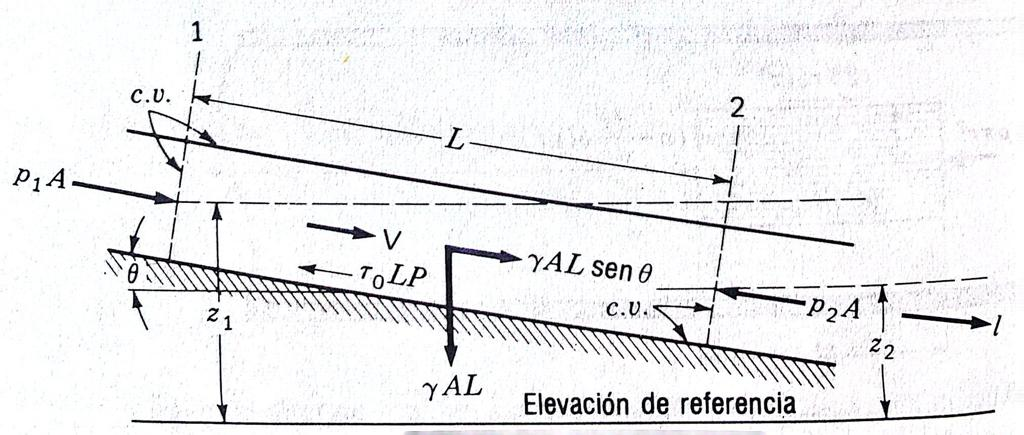
\includegraphics[width=8cm]{perd.jpeg}
\caption{Fuerzas axiales sobre un volumen de control en un conducto (tomado de \cite{streeter}).}
\label{perd}
\end{figure}

Las p\'erdidas de energ\'ia entre dos secciones 1 y 2 en conductos se puede expresar usando la ecuaci\'on de energ\'ia a partir de la ecuaci\'on de la \emph{ecuaci\'on de Bernoulli} (ecuaci\'on~\ref{bernu}):

\begin{equation}
\color{red}\boxed{\color{black} \frac{p_1}{\gamma} + \frac{V_1^2}{2g} + z_1 = \frac{p_2}{\gamma} + \frac{V_2^2}{2g} + z_2 + h_{1-2}  }
\label{perd1}
\end{equation}

donde $h_{1-2}$ son las p\'erdidas de energ\'ia entre 1 y 2. Como la secci\'on transversal en el conducto es constante, el termino $\frac{V^2}{2g}$ se elimina a ambos lados, por lo que las perdidas se expresan como:
 
\begin{equation}
h_{1-2} = \frac{p_1 - p_2}{\gamma} + z_1 - z_2
\label{perd2}
\end{equation}

Note que las p\'erdidas son proporcionales a los cambios en la cabeza de presi\'on y en la energ\'ia potencial.

De acuerdo con la ecuaci\'on de conservaci\'on de la cantidad de movimiento lineal para  el volumen de control de la  figura~\ref{perd} en la direcci\'on del flujo $l$, tenemos:

\begin{equation}
\sum F_l = 0 = (p_1 - p_2)A + \gamma AL \sin \theta - \tau_0 L P
\label{perd3}
\end{equation}

donde $L$ es la distancia entre 1 y 2, $A$ es el \'area de la secci\'on transversal en 1 y en 2, $P$ es el \emph{per\'imetro mojado} de la secci\'on, el cual es la porci\'on de la secci\'on transversal en contacto con el fluido excluyendo la superficie libre. Teniendo en cuenta que $L\sin \theta = z_1 - z_2$, se tiene:
 
\begin{equation}
\frac{p_1 - p_2}{\gamma} + z_1 - z_2 = \frac{\tau_0 L P}{\gamma A}
\label{perd4}
\end{equation}

Igualando las ecuaciones~\ref{perd2} y ~\ref{perd4} y usando la ecuaci\'on~\ref{perd0}, se tiene:

\begin{equation}
h_{1-2} = \frac{\tau_0 LP}{\gamma A} = \lambda \frac{\rho}{2}V^2 \frac{LP}{\gamma A} =\lambda \frac{L}{R} \frac{V^2}{2g}
\label{perd5}
\end{equation}

donde $R$ es el radio hidr\'aulico del conducto $R = \frac{A}{P}$, para una tuber\'ia $R= \frac{D}{4}$ donde $D$ es el di\'ametro del tubo. Note que el las perdidas de energ\'ia $h_{1-2}$ tiene unidades de Newton-metro por newton o libras-pie por libra. Teniendo en cuenta que las p\'erdidas de cabeza de energ\'ia son debido a la fricci\'on, $h_{1-2} = h_f$. Si se expresan $h_f$ en t\'erminos de longitud, se tiene que la \emph{pendiente de la l\'inea de energ\'ia} $S$ se expresa:

\begin{equation}
S = \frac{h_f}{L} = \frac{\lambda}{R}\frac{V^2}{2g} 
\label{perd6}
\end{equation}

Despejando la velocidad $V$ de la ecuaci\'on~\ref{perd6}:

\begin{equation}
\color{red}\boxed{\color{black} V = \sqrt{\frac{2g}{\lambda}}\sqrt{RS} = C \sqrt{RS} }
\label{perd7}
\end{equation}

donde $C$ es un coeficiente de fricci\'on que depende de la rugosidad del material y del tama\~no del conducto y se encuentra de manera experimental. La ecuaci\'on~\ref{perd7} es conocida como la \emph{ecuaci\'on de Chezy} y $C$ es el \emph{coeficiente de Chezy}. Existen diferentes formulas para calcular $C$, para tuber\'ias se tiene que $\lambda = f/4$, reemplazando en la ecuaci\'on~\ref{perd5}, se tiene:

\begin{equation}
\color{red}\boxed{\color{black} h_f = f \frac{L}{D} \frac{V^2}{2g}}
\label{perd8}
\end{equation}

donde $f$ es el \emph{factor de fricci\'on} que se ha determinado experimentalmente para tuber\'ias. Esta ecuaci\'on es aplicable a conductos abiertos (canales) de la siguiente forma:

\begin{equation}
V = \sqrt{\frac{8g}{f}}\sqrt{RS}
\label{perd9}
\end{equation}

\subsection{C\'alculo del factor de fricci\'on} % From Duarte
Al hacer un analisis del flujo turbulento, las variables que influyen en su comportamiento son: la velocidad media del flujo $V$ [$L T^{-1}$], la viscosidad din\'amica  $\mu$ [$ML^{-1} T^{-1}$] o cinem\'atica $\nu$ [$L^{2} T^{-1}$], la densidad del fluido $\rho$ [$M L^{-3}$], el esfuerzo de corte en la pared $\tau_0$ [$ML^{-1} T^{-2}$], una longitud caracter\'istica $L_c$ que para el caso espec\'ifico de flujo en tuber\'ias de secci\'on transversal circular es igual a $D$ [$L$] y la rugosidad absoluta del tubo $\varepsilon$ [$L$]. De acuerdo con esto, podemos decir que en el flujo turbulento intervienen 6 variables y 3 dimensiones fundamentales: masa $M$, longitud $L$ y tiempo $T$. Utilizando el \emph{teorema Pi de Buckingham} y el analisis dimensional se puede obtener una ecuaci\'on que relacione estas 6 variables: $f(\tau_0, \rho, \mu, \nu, D, V, \varepsilon)=0$. De acuerdo con el teorema, si el numero de variables $n=6$ y el numero de dimensiones $m=3$, el n\'umero de parametros adimensionales es $n-m=3$. Aplicando el teorema y tomando como variables repetit\'ivas $\varepsilon$, $\rho$ y $V$,  los par\'ametros adimensionales son: 

\begin{equation}
\Pi_1 = \frac{\rho V D}{\mu} = Re \hspace{2cm}  \Pi_2 = \frac{\rho V^2}{\tau_0} = E \hspace{2cm} \Pi_3 = \frac{\varepsilon}{D} 
\label{fric1}
\end{equation}

donde $E$ es el \emph{n\'umero de Euler}. De acuerdo con lo anterior, $f(Re, E, \varepsilon/D)=0$ o  $\frac{\rho V^2}{\tau_0} = f(Re,\varepsilon/D)$. Despejando $\tau_0$, se tiene:

\begin{equation}
\tau_0 = \rho V^2 \left[ f \left(Re , \frac{\varepsilon}{D} \right) \right]
\label{fric2}
\end{equation}

Note que al despejar $ f \left(Re , \frac{\varepsilon}{D}\right)^{-1}$ es equivalente a $f \left(Re , \frac{\varepsilon}{D}\right)$ ya que $f$ es funci\'on de variables adimensionales. De la ecuaci\'on~\ref{perd5},  $\tau_0 = \frac{h_f \gamma R}{L} = \frac{h_f \rho g D}{4L}$ igualando esta expresi\'on a la ecuaci\'on~\ref{fric2} y simplificando, se tiene:

\begin{equation}
h_f = \frac{L}{D}\frac{V^2}{2g} \left[8 f \left(Re , \frac{\varepsilon}{D} \right) \right]
\label{fric3}
\end{equation}

Note que el t\'ermino entre par\'entesis en la ecuaci\'on~\ref{fric3} es una funci\'on de $Re$ y $\varepsilon/D$, es el factor de fricci\'on (ver ecuaci\'on~\ref{perd8}), por lo que la ecuaci\'on~\ref{fric3} se convierte en:

\begin{equation}
\color{red}\boxed{\color{black} h_f = f \frac{L}{D} \frac{V^2}{2g}}
\label{fric4}
\end{equation}

la cual es conocida como la \emph{ecuaci\'on de Darcy-Weisbach}. Esta ecuaci\'on se puede aplicar al flujo laminar y al flujo turbulento, sin embargo, el factor de fricci\'on en flujo turbulento depende no solo de $Re$ si no de la rugosidad $\varepsilon$ del contorno.

Existen diferentes  ecuaciones para definir el valor del coeficiente de fricci\'on dependiendo de si la superficie del conducto es lisa o rugosa. Estas ecuaciones han sido derivadas de an\'alisis experimentales por diferentes investigadores como Blassius, Prandtl, Von Karman, Nikuradse, Jain, etc.

Blasius encontr\'o que, para superficies hidr\'aulicamente lisas y flujo turbulento en el rango $4000 < Re < 100000$, $f$ se calcula como:

\begin{equation}
\color{red}\boxed{\color{black} f = \frac{0.316}{Re^{0.25}} }
\label{fric5}
\end{equation}

Nikuradse realiz\'o experimentos usando tres tuber\'ias con diferente di\'ametro a las cuales les adher\'ia uniformemente granos de arena de diferente di\'ametro ($\varepsilon$). Nikuradse encontr\'o (ver figura~\ref{nikur}) que cuando la rugosidad relativa $\varepsilon/D$ variaba desde 0.001 hasta 0.033, $f$ presentaba un comportamiento complejo que depend\'ia del n\'umero de Reynolds y de la condici\'on hidrodin\'amica del contorno. De los experimentos de Nikuradse, se encontr\'o:

% Fig 5.20 Streeter 
\begin{figure}[h]
\centering
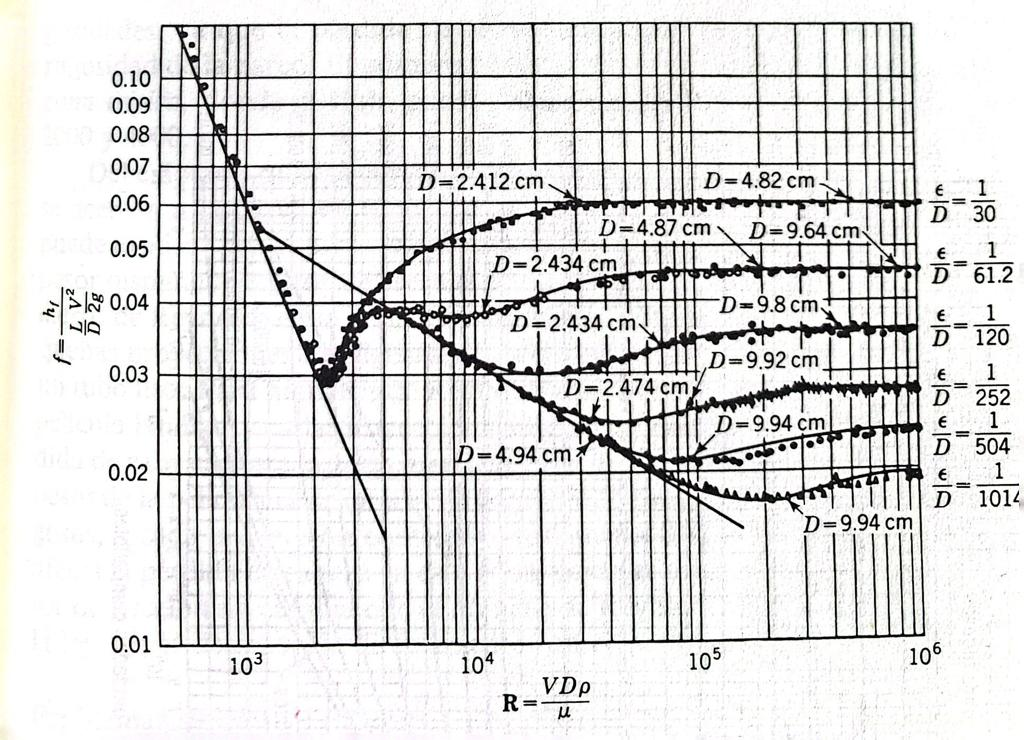
\includegraphics[width=8cm]{nikur.jpeg}
\caption{Experimentos de Nikuradse con tubos con rugosidades formadas con diferentes di\'ametros de arena (tomado de \cite{streeter}).}
\label{nikur}
\end{figure}

\begin{itemize}
\item Para flujo laminare ($Re<2100$) los datos experimentales definen una l\'inea que satisface la ecuaci\'on~\ref{fric4}, donde: 

\begin{equation}
\color{red}\boxed{\color{black} f = \frac{64}{Re} }
\label{fric6}
\end{equation}

\item Para flujo turbulento ($Re > 4000$), los datos experimentales muestran una serie de curvas (ver figura~\ref{nikur}) definidas por $\varepsilon/D$, por lo que $f$ es una funci\'on de $Re$ y de la rugosidad del tubo. En esas curvas se pueden definir tres zonas:

\begin{enumerate}
\item Una primera zona definida por una curva envolvente para superficies lisas ($\delta > \varepsilon$), por lo que $f$ es independiente de la rugosidad.
\item Una segunda zona en donde las curvas de $f$ vs $Re$ son paralelas para diferentes valores de $\varepsilon/D$, lo que evidencia que $f$ es independiente de $Re$; si $Re$ aumenta el valor de $f$ permanece constante. Esta zona define las superficies hidr\'aulicamente rugosas y es conocida como la \emph{zona totalmente rugosa}. El espesor de la capa viscosa $\delta '$ disminuye a medida que incrementa $Re$.
\item Una tercera zona que define las superficies lisas (envolvente inferior). Se conoce como \emph{zona rugosa de transici\'on}. 
\end{enumerate}
\end{itemize}
  
Teniendo en cuenta el comportamiento de $f$, Prandtl y Von Karman presentaron las siguientes ecuaciones las cuales se ajustan muy bien a los datos experimentales obtenidos por Nikuradse:
\begin{itemize}
\item Para $Re > 4000$ y tuber\'ias lisas

\begin{equation}
\color{red}\boxed{\color{black} \frac{1}{\sqrt{f}} = 0.869 \ln \left( Re \sqrt{f} \right ) - 0.8 }
\label{fric7}
\end{equation}

\item Para $Re > 4000$ y tuber\'ias rugosas 

\begin{equation}
\color{red}\boxed{\color{black} \frac{1}{\sqrt{f}} = 1.14 - 0.869 \ln \left( \frac{\varepsilon}{D} \right ) }
\label{fric8}
\end{equation}

\end{itemize}

Sin embargo, teniendo en cuenta que los experimentos de Nikuradse se realizaron para tuber\'ias con granos de arena adheridos uniformemente a las paredes de la tuber\'ia, dicha condici\'on dista mucho de la realidad en donde ni la rugosidad ni el di\'ametro son uniformes. Para estudiar el comportamiento en tuber\'ias comerciales en donde la rugosidad es irregular, C.F. Colebrook(1939), realiz\'o experimentos con el prop\'osito de mostrar la aplicabilidad de las ecuaciones~\ref{fric7} y ~\ref{fric8}. Colebrook obtuvo que en la zona de transici\'on, existe un efecto de la no uniformidad de la rugosidad $\varepsilon$. Para tuber\'ias comerciales de secci\'on circular, Colebrook obtuvo una ecuaci\'on implicita para $f$ para la zona de transici\'on:

\begin{equation}
\color{red}\boxed{\color{black} \frac{1}{\sqrt{f}}= -2 \log \left( \frac{\varepsilon}{3.7D} + \frac{2.52}{Re \sqrt{f}} \right) }
\label{fric9}
\end{equation}

En t\'erminos de caudal $Q$, $Re = \frac{QD}{A \nu} = \frac{4Q}{\pi D \nu}$, la ecuaci\'on~\ref{fric9} se expresa como:

\begin{equation}
\color{red}\boxed{\color{black} f  = \left[ -2 \log \left( \frac{\varepsilon}{3.7D} + \frac{1.979 \nu D}{Q \sqrt{f}} \right) \right]^{-2} }
\label{fric10}
\end{equation}

L.F. Moody present\'o un diagrama (ver figura~\ref{mood}) para determinar el factor de fricci\'on $f$ en tuber\'ias comerciales para flujos laminares y turbulento con base en las ecuaciones~\ref{fric5}, ~\ref{fric7}, ~\ref{fric8} y \ref{fric9}. El \emph{diagrama de Moody} sirve para determinar $f$ en funci\'on de $Re$ y $\varepsilon/D$. EL diagrama presenta una serie de curvas que definen el comportamiento de flujo: laminar ($Re<2100$, l\'inea recta con pendiente -1) de transici\'on y turbulento ($Re>4000$).  La zona de flujo turbulento esta compuesta por tres zonas: superficies hidr\'aulicamente lisas en donde $f$ depende solamente de $Re$, superficies en transici\'on de lisas a rugosas donde $f$ depende de $Re$ y de $\varepsilon/D$ y superficie hidr\'aulicamente rugosa donde $f$ depende de $\varepsilon/D$ solamente. 

% Fig 6.13 White 
\begin{figure}[h]
\centering
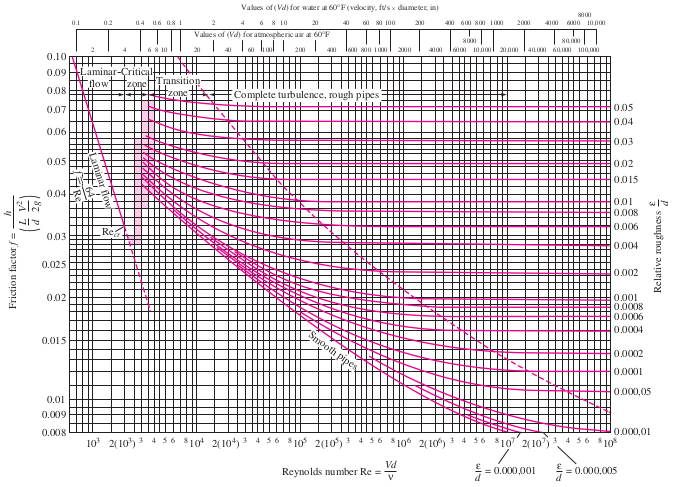
\includegraphics[width=8cm]{mood.png}
\caption{Diagrama de Moody para tuber\'ias comerciales con flujo laminar y turbulento (tomado de \cite{white1990fluid}).}
\label{mood}
\end{figure}

El diagrama de Moody t\'ambien puede ser utilizado en flujo a superficie libre (e.g. canales) utilizando el radio hidr\'aulico $R$ en lugar del di\'ametro $D$. 

En 1976, Swanee y Jain presentaron una ecuaci\'on explicita para el factor $f$ como:

\begin{equation}
\color{red}\boxed{\color{black} f  = 0.25 \left[ \log \left( \frac{\varepsilon}{3.7D} + \frac{5.74}{Re^{0.9}} \right) \right]^{-2} }
\label{fric11}
\end{equation}

Esta ecuaci\'on es valida para los siguientes rangos de n\'umero de Reynolds y de rugosidad relativa $\varepsilon/D$: $4000<Re<1x10^8 $ y $0.01<\varepsilon/D <1x10^{-4}$.


% Ej 5.9 Duarte
\begin{shaded}
\begin{exa}
Fluye petroleo ($S=0.8$, $\mu = 0.0052$ Pa.s) a trav\'es de una tuber\'ia de 10 cm de di\'ametro y rugosidad $\varepsilon=0.85$ mm a raz\'on de 40 l/s. Determinar la disipaci\'on de energ\'ia por unidad de longitud en la tuber\'ia y el esfuerzo de corte en la pared del conducto. Encontrar la magnitud de la velocidad a una distancia radial de 2 cm desde el centro de la tuber\'ia. Definir si la superficie se comporta como hidraulicamente lisa, en transici\'on o rugosa.
\end{exa}
\end{shaded}

% Ej 8-3 Cengel
\begin{shaded}
\begin{exa}
Agua a 60 $^o$F ($\rho=62.36$ lbm/ft$^3$ y $\mu = 7.536 x10^{-4}$ lbm/ft.s ) fluye a trav\'es de una tuber\'ia de acero ($\varepsilon= 7x10^{-6}$ft) horizontal de 2 in de diametro y longitud 200 ft con un caudal 0.2 ft$^3$/s. Determinar la caida de la cabeza de presi\'on, la perdida de energ\'ia y la potencia requerida para bombear agua a trav\'es de la tuber\'ia. 
\end{exa}
\end{shaded}



%Similarmente, en 1976 Swanee and Jain presentaron la siguiente ecuaci\'on para el factor de fricci\'on $f$:
%
%\begin{equation}
%\color{red}\boxed{\color{black} f  = 0.25 \left[  \log \left( \frac{\varepsilon}{3.7D} + \frac{5.74}{Re^{0.9}} \right) \right]^{-2} }
%\label{fric11}
%\end{equation}
%
%la cual es valida para $4000<Re< 1x10^8$ y $0.01< \varepsilo/D < 1$ 

\subsection{Otras ecuaciones para calcular las p\'erdidas de energ\'ia} % From Duarte
\subsubsection*{Ecuaci\'on de Hazen-Williams}
Hazen y Williams presentaron la siguiente expresi\'on para la velocidad media del agua en r\'egimen turbulento:

\begin{equation}
\color{red}\boxed{\color{black} V = 0.85 C_H R^{0.63} S_f^{0.54} }
\label{other0}
\end{equation}

donde $V$ es la velocidad media en m/s, $C_H$ es un coeficiente de rugosidad que depende del material de la tuber\'ia (ver tabla~\ref{hwi}), $R$ es el radio hidr\'aulico en m y $S_f$ es la pendiente de la l\'inea de energ\'ia $S_f = h_f / L$, donde $L$ es la longitud en m.

\begin{table}[h!]
\centering
\begin{tabular}{l c}
 \hline
 Material del conducto & $C_H$ \\ [0.5ex]
 \hline\hline
PVC & 150 \\
Fundici\'on asfaltada & 140 \\
Eternit - Asbesto - Cemento & 140 \\
Acero & 130$-$140 \\
Hierro Forjado & 130$-$140 \\
Fundici\'on & 130 \\
Hormig\'on & 120 \\
Acero liso & 120 \\
Madera & 120 \\
Fibra de vidrio & 110 \\
%Fundici\'on en malas condiciones 
\hline
\end{tabular}
\caption{Coeficientes de rugosidad de Hazen-Williams, $C_H$ (tomado de \cite{agudelo2011mecanica}).}
\label{hwi}
\end{table}

Teniendo en cuenta que para tuber\'ias de secci\'on circular donde $R=D/4$, la ecuaci\'on~\ref{other0} se puede expresar en t\'erminos de $h_f$ como:

\begin{equation}
h_f = 10.654 L \left[ \frac{Q}{C_H D^{2.63}} \right]^{1.85}
\label{other1}
\end{equation}

donde $Q$ es el caudal a trav\'es del conducto en m$^3$/s.

\subsubsection*{Ecuaci\'on de Manning}
Robert Manning en 1880 obtuvo una expresi\'on en el sistema Ingl\'es de unidades para determinar la velocidad media del agua en tuber\'ias:

\begin{equation}
\color{red}\boxed{\color{black} V = \frac{1.49}{\eta} R^{\frac{2}{3}} S_f^{\frac{1}{2}} }
\label{other2}
\end{equation}

donde $\eta$ es un coeficiente de rugosidad que depende del material del conducto y de las propiedades hidr\'aulicas del flujo. Despejando de la ecuaci\'on~\ref{other2} las p\'erdida de energ\'ia $h_f$ y expresandola en sistema internacional, se tiene:

\begin{equation}
h_f = \frac{10.29 L \eta^2 Q^2}{D^{16/3}}
\label{other3}
\end{equation}

Al observar las ecuacione~\ref{other1} y \ref{other3}, se puede afirmar que la disipaci\'on o p\'erdida de energ\'ia se puede expresar de manera general como:

\begin{equation}
h_f = C Q^n
\label{other4}
\end{equation}

donde $C$ es una constante que depende de un sistema de unidades, longitud, di\'ametro y rugosidad del conducto, y el exponente $n$ varia entre 1.0 y 2.0 depende del r\'egimen de flujo. La tabla~\ref{tper} define el valor de $C$  y de $n$ en la ecuaci\'on~\ref{other4} para el sistema Internacional y para el sistema Ing\'es de unidades. 

\begin{table}[h!]
\centering
\begin{tabular}{l c c}
 \hline
 & Sistema Internacional & Sistema Ing\'es \\ [0.5ex]
 & L(m), D(m), Q(m$^3$/s) & L(pie), D(pie), Q(pie$^3$/s) \\ [0.5ex]
 \hline\hline
Ecuaci\'on de Darcy-Weisbach (n=2) & $C=0.0827 f\frac{L}{D^5}$ &  $C=0.0252 f\frac{L}{D^5}$\\
Ecuaci\'on de Hazen-Williams (n=1.85) & $C=10.654 L \left[ \frac{1}{C_H D^{2.63}}\right]^{1.85}$ &  $C=4.72 L \left[ \frac{1}{C_H D^{2.63}}\right]^{1.85}$ \\
\hline
\end{tabular}
\caption{Ecuaciones para la disipaci\'on de energ\'ia $h_f = C Q^n$ (tomado de \cite{agudelo2011mecanica}).}
\label{tper}
\end{table}


\section{P\'erdidas menores} % From Cengel and Duarte
En un sistema de tuber\'ias, el flujo pasa a trav\'es de m\'ultiples \emph{entradas, salidas, uniones, v\'alvulas, codos, bifurcaciones, expansiones, contracciones, etc} (ver figura~\ref{acce}) en adici\'on de los tramos rectos de las tuber\'ias. Estos componentes del sistema causan separaci\'on y mezcla del flujo induciendo p\'erdidas de energ\'ia adicional. Comparadas con las perdidas por fricci\'on, $h_f$, las p\'erdidas debido a estos accesorios, $h_e$, son menores. Sin embargo, en algunos casos en donde existen muchos cambios de direcci\'on y v\'alvulas en un tramo corto de tuber\'ia,  $h_e$ llega a ser mayor que $h_f$. Cuando una v\'alvula esta totalmente abierta la p\'erdidas de energ\'ia a trav\'es de esta son despreciable. Sin embargo cuando la v\'alvula esta parcialmente abierta, existen p\'erdidas de energ\'ia debido a la disminuci\'on de caudal a trav\'es de la v\'alvula. 


% Fig 5.26 Duarte 
\begin{figure}[h]
\centering
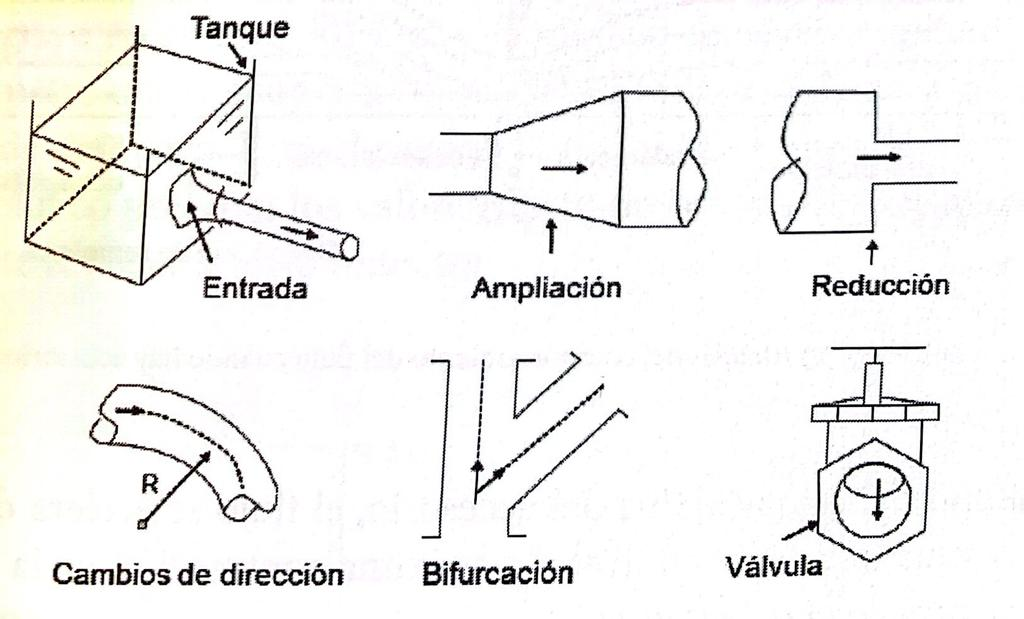
\includegraphics[width=8cm]{acce.jpeg}
\caption{Accesorios de uso com\'un en tuber\'ias (tomado de \cite{agudelo2011mecanica}).}
\label{acce}
\end{figure}

La cuantificaci\'on de las p\'erdidas menores es complejo desde el punto de vista te\'orico. Por esto, estas p\'erdidas son determinadas experimentalmente por los fabricantes de los accesorios. Las p\'erdidas menores, $h_e$, son expresadas usualmente como:

\begin{equation}
\color{red}\boxed{\color{black} h_e = K \frac{V^2}{2g} }
\label{perm0}
\end{equation}

donde $K$ es el \emph{coeficiente de p\'erdida o de resistencia} que depende del n\'umero de Reynolds, del material del cual esta hecho el accesorio y de la forma como se acopla el accesorio. Sin embargo, para $Re > 10^5$ se ha demostrado que $K$ es independiente del n\'umero de Reynolds.

Vennard-Street explican  f\'isicamente el efecto de un accesorio sobre la energ\'ia disponible en el sistema y sobre el flujo. Dichos efectos se analizando mediante la figura~\ref{acce1}:

% Fig 5.27 Duarte 
\begin{figure}[h]
\centering
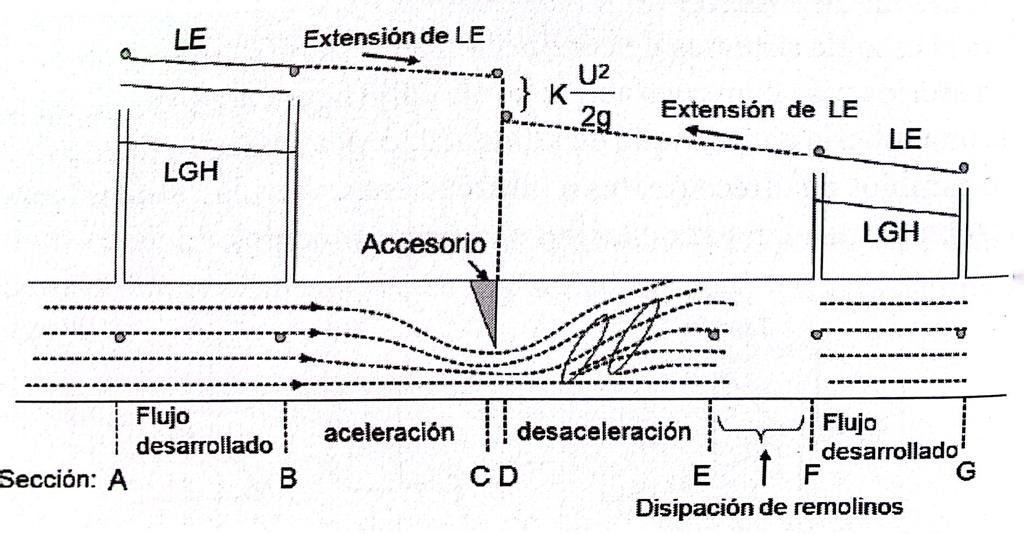
\includegraphics[width=8cm]{acce1.jpeg}
\caption{Comportamiento del flujo en una tuber\'ia con accesorio (tomado de \cite{agudelo2011mecanica}).}
\label{acce1}
\end{figure}

\begin{itemize}
\item \textbf{Zona BC}: Aguas arriba del accesorio, la vena l\'iquida se contrae y el flujo se acelera. La m\'axima contracci\'on de la vena liquida se presenta justo en la posici\'on del accesorio o un poco aguas abajo de este. Debido a la contracci\'on, la presi\'on disminuye. 
\item \textbf{Zona DE}: En esta zona la presi\'on del flujo aumenta ya que la velocidad del  disminuye. El flujo se desacelera generando la creaci\'on de remolinos que ocacionan una turbulencia de gran escala. Por lo tanto una parte de la energ\'ia se pierde debido a la creaci\'on de remolinos. 
\item \textbf{Zona EF}: En esta zona se disipan (desaparecen) los remolinos. Aguas abajo de esta zona se restablece la condici\'on de flujo desarrollado.
\end{itemize}

Note que a lo largo de la longitud AG (ver figura~\ref{acce1}) t\'ambien act\'uan las fuerzas de fricci\'on. Dichas p\'erdidas debido a la fricci\'on se calculan asumiendo flujo desarrollado a lo largo de AG. Las p\'erdidas globales a lo largo de AG son entonces la suma de las p\'erdidas debido al accesorio (p\'erdidas locales entre C y D) y debido a la fricci\'on (a lo largo de AG). Las \emph{p\'erdida total} de energ\'ia en un sistema puede expresarse como:
  
\begin{equation}
\color{red}\boxed{\color{black} h_T = \sum_{i} {h_f}_i + \sum_{j} {h_e}_j =\sum_{i} f_i \frac{L_i }{D_i} \frac{V_i^2}{2g} + \sum_{j} K_j \frac{{V_j}^2}{2g} }
\label{perm1}
\end{equation}

donde $i$ representa cada tuber\'ia con di\'ametro constante y $j$ representa cada componente que causa una p\'erdida menor. Si el sistema analizado tiene di\'ametro constante y del mismo material, la ecuaci\'on~\ref{perm1}, se convierte en:

\begin{equation}
\color{red}\boxed{\color{black} h_T = \left( f \frac{L }{D} + \sum_{j} K_j \right) \frac{V^2}{2g} }
\label{perm2}
\end{equation}

donde $V$ es la velocidad media en todo el sistema. 

Los sistemas de tuber\'ias comunmente contienen \emph{contracciones o expansiones subitas o graduales} de la secci\'on de la tuber\'ia con el fin de acomodar cambios de caudal o velocidad o de propiedades del fluido (e.g. densidad). Las p\'erdidas son usualmente mayores cuando los cambios son s\'ubitos o con un \'angulo grande debido a la separaci\'on del flujo (ver figura~\ref{acce2}).

% Fig 3.40 Streeter 
\begin{figure}[h]
\centering
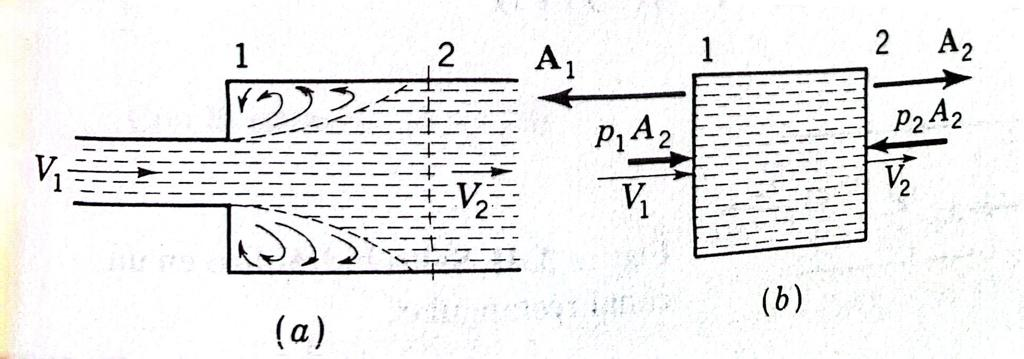
\includegraphics[width=8cm]{acce2.jpeg}
\caption{Representaci\'on de la p\'erdida de energ\'ia en una expansi\'on subita. (tomado de \cite{streeter}).}
\label{acce2}
\end{figure}

Aplicando la ley de conservaci\'on de cantidad de movimiento para el volumen de control en la figura~\ref{acce2} entre las secci\'on 1 y 2, tenemos:

\begin{equation}
p_1 A_2 - p_2 A_2 = \rho V_2 (V_2 A_2) + \rho V_1 (-V_1 A_1 )
\label{perm3}
\end{equation}

teniendo en cuenta que de acuerdo con la ley de continuidad $V_1 A_1 = V_2 A_2$, y despejando $\frac{p_1 - p_2}{\gamma}$ de la ecuaci\'on~\ref{perm3}, se tiene que:

\begin{equation}
\frac{p_1 - p_2}{\gamma} =  \frac{{V_2}^2 - V_2 V_1}{g}
\label{perm4}
\end{equation}

Aplicando la ley de conservaci\'on de la energ\'ia entre las secciones 1 y 2 en la figura~\ref{acce2}, se tiene:

\begin{equation}
\frac{{V_1}^2}{2g} + \frac{p_1}{\gamma} = \frac{{V_2}^2}{2g} + \frac{p_2}{\gamma} + h_e
\label{perm5}
\end{equation}

despejando $\frac{p_1 - p_2}{\gamma}$ de la ecuaci\'on~\ref{perm5} e igualando a la ecuaci\'on~\ref{perm4}, se tiene:

\begin{equation}
\frac{{V_2}^2 - V_2 V_1}{g} = \frac{{V_2}^2 - {V_1}^2}{2g} + h_e
\label{perm6}
\end{equation}

despejando $h_e$ de la ecuaci\'on~\ref{perm6} y usando la ecuaci\'on de continuidad, se tiene:

\begin{equation}
\color{red}\boxed{\color{black} h_e = \frac{(V_1 - V_2)^2}{2g} = \frac{{V_1}^2}{2g}\left( 1- \frac{A_1}{A_2} \right)^2 }
\label{perm7}
\end{equation}

La ecuaci\'on~\ref{perm7} determina la p\'erdidas locales en una expansi\'on brusca, por lo que:

\begin{equation}
\color{red}\boxed{\color{black} K = \left( 1- \frac{A_1}{A_2} \right)^2 }
\label{perm8}
\end{equation}

Note que la ecuaci\'on~\ref{perm7} representa la deducci\'on de una expresi\'on para calcular las p\'erdidas menores en t\'erminos generales teniendo en cuenta que afirma que las p\'erdidas menores varian con el cuadrado de la velocidad afectada por un coeficiente $K$, que como lo hab\'iamos afirmado, esta dado generalmente por el fabricante. 

Analizando la ecuaci\'on~\ref{perm8}, en el caso en que la tuber\'ia descargue a un deposito ($A_1 << A_2$),  $K \approx 1$ lo que significa que la energ\'ia cin\'etica del flujo se convierte en energ\'ia t\'ermina (calor).  

Para el caso de la contracci\'on brusca que se muestra en la figura~\ref{contr}, se hace un an\'alisis similar al realizado para el caso de la expansi\'on brusca. Partiendo de la ecuaci\'on~\ref{perm7}, se tiene:

% Fig 5.23 Streeter 
\begin{figure}[h]
\centering
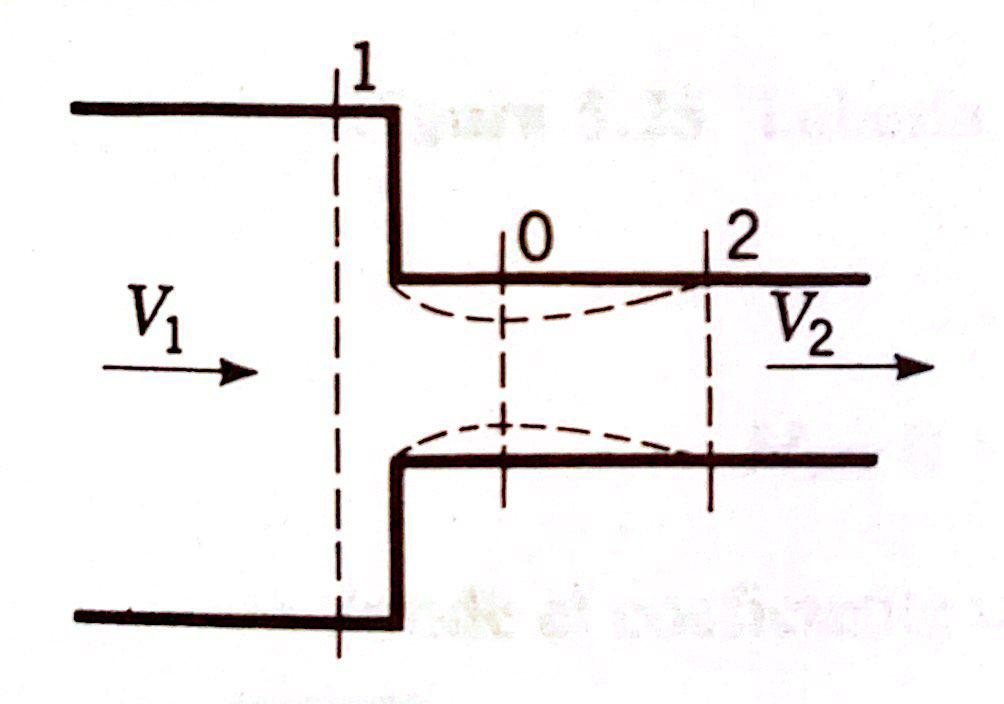
\includegraphics[width=8cm]{contr.jpeg}
\caption{Contracci\'on brusca en una tuber\'ia (tomado de \cite{streeter}).}
\label{contr}
\end{figure}

\begin{equation}
h_e = \frac{(V_0 - V_2)^2}{2g} 
\label{perm9}
\end{equation}

Teniendo en cuenta la vena l\'iquida contra\'ida en la secci\'on 0, la ecuaci\'on de continuidad entre 0 y 2 es $V_0 C_c A_2 = V_2 A_2$ en donde $C_c$ es un coeficiente de contracci\'on que fue determinado inicialmente por Weisbach con respecto a la relaci\'on $A_2 /A_1$. Reemplazando en la ecuaci\'on~\ref{perm9}, se tiene:

\begin{equation}
\color{red}\boxed{\color{black} h_e = \left( \frac{1}{C_c} -1 \right)^2 \frac{{V_2}^2}{2g} = K  \frac{{V_2}^2}{2g} }
\label{perm10}
\end{equation}

En las figuras~\ref{acce3} y ~\ref{acce4} se presentan valore de $K$ para diferentes tipos de accesorios. 

% Fig 8-4 Cengel 
\begin{figure}[h]
\centering
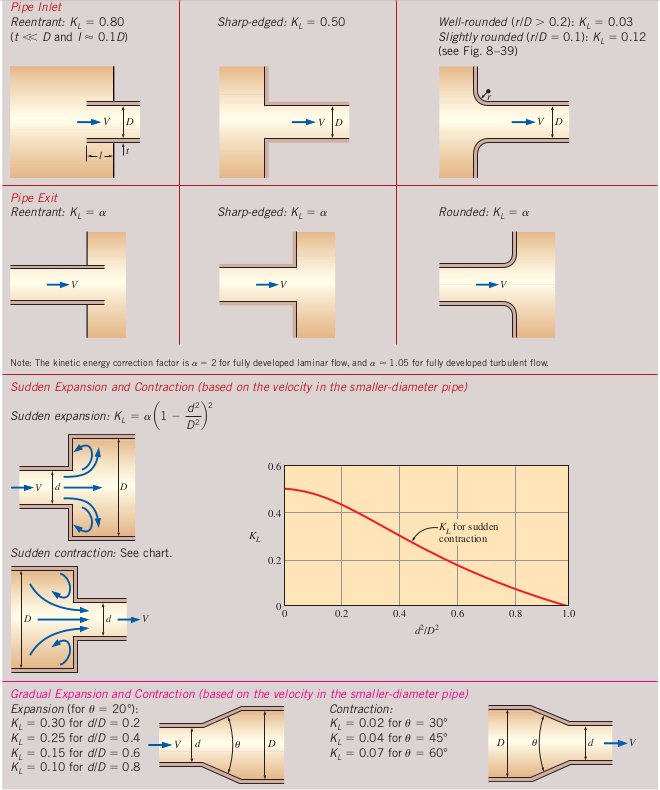
\includegraphics[width=8cm]{acce3.png}
\caption{Valores de $K$ para diferentes tipos de accesorios para flujo turbulento (tomado de \cite{cengel2013ebook}).}
\label{acce3}
\end{figure}

% Fig 8-4 Cengel 
\begin{figure}[h]
\centering
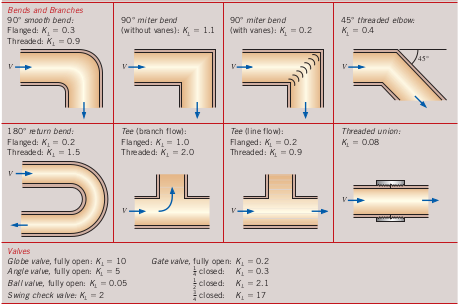
\includegraphics[width=8cm]{acce4.png}
\caption{Valores de $K$ para diferentes tipos de accesorios para flujo turbulento (tomado de \cite{cengel2013ebook}).}
\label{acce4}
\end{figure}

\subsection{Longitud equivalente} % From  Streeter
Las p\'erdidas menores se pueden expresar en t\'erminos de la longitud equivalente $L_e$ de tubo con la misma p\'erdida de cabeza para el mismo caudal as\'i:

\begin{equation}
f \frac{L_e }{D} \frac{V^2}{2g} = K \frac{V^2}{2g}
\label{perm11}
\end{equation}

en donde $K$ puede referirse a una p\'erdida de carga menor o a la suma de varias p\'erdidas. Al despejar $L_e$, se tiene:

\begin{equation}
\color{red}\boxed{\color{black} L_e = \frac{KD}{f} }
\label{perm12}
\end{equation}

Por ejemplo, si las p\'erdidas menores en una tuber\'ia de $12\ pulg = 1\ ft$ se suman y da $K=20$, y si $f = 0.020$ para la tuber\'ia, a la longitud real de la tuber\'ia se puede sumar $20(1/0.020)=1000 ft$ y esta longitud adicional o equivalente causa la misma resistencia al flujo que las p\'erdidas menores. 

% Ej 5.13 Streeter
\begin{shaded}
\begin{exa}
Encu\'entrese el caudal que fluye por la tuber\'ia en la figura con $H =$ 10 $m$, y H para un caudal de 60 $L/s$.
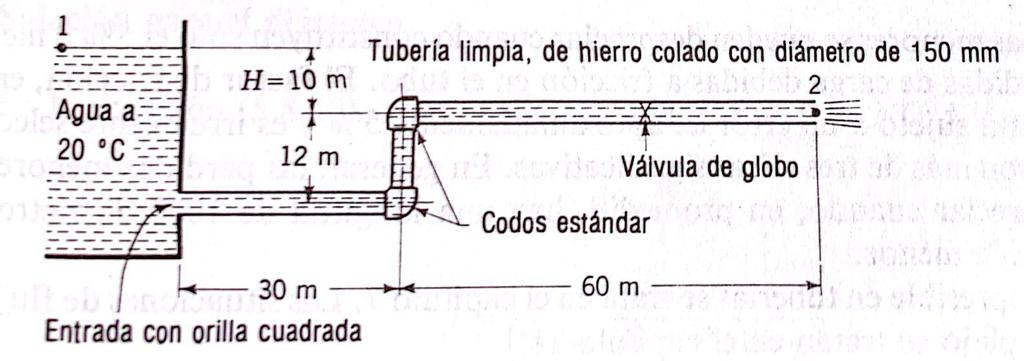
\includegraphics[width=8cm]{exa20.jpeg}
\end{exa}
\end{shaded}


% Ej 5.11 Duarte 
\begin{shaded}
\begin{exa}
Por un sistema de conducci\'on de un modelo de laboratorio, fluye agua con un caudal de 0.0014 $m^3/s$. El modelo consiste en una tuber\'ia de 25 $mm$ de di\'ametro que se acopla, a trav\'es de una reducci\'on brusca, a una tuber\'ia de 19 $mm$ de di\'ametro. Para el caudal ya definido, la l\'inea resultante de gradiente hidr\'aulico presenta los valores ilustrados en la figura. Determinar el coeficiente $K$ del accesorio reductor.
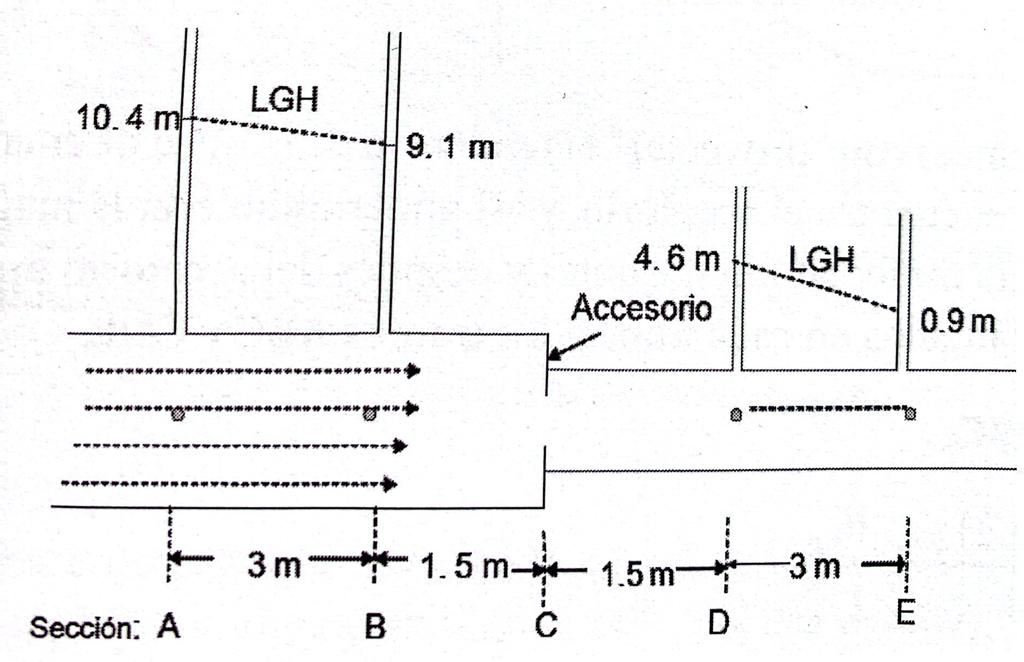
\includegraphics[width=8cm]{exa30.jpeg}
\end{exa}
\end{shaded}

% REFERENCES
\bibliographystyle{plain} % We choose the "plain" reference style
\bibliography{refs} % Entries are in the refs.bib file

\end{document}
